\documentclass[pdflatex,sn-mathphys-ay]{sn-jnl}

\usepackage[T1]{fontenc}%
\usepackage{graphicx}%
\usepackage{multirow}%
\usepackage{amsmath,amssymb,amsfonts}%
\usepackage{amsthm}%
\usepackage{mathrsfs}%
\usepackage[title]{appendix}%
\usepackage{xcolor}%
\usepackage{textcomp}%
\usepackage{manyfoot}%
\usepackage{booktabs}%
\usepackage{array}%
\usepackage{longtable}%
\usepackage{calc}%
\usepackage{newunicodechar}%
\usepackage{fvextra}%
\providecommand{\tightlist}{\setlength{\itemsep}{0pt}\setlength{\parskip}{0pt}}
\providecommand{\lt}{<}\providecommand{\gt}{>}
\newunicodechar{§}{\S}
\newunicodechar{→}{\ensuremath{\rightarrow}}
\newunicodechar{↔}{\ensuremath{\leftrightarrow}}
\newunicodechar{×}{\ensuremath{\times}}
\newunicodechar{·}{\ensuremath{\cdot}}
\newunicodechar{⊃}{\ensuremath{\supset}}
\newunicodechar{°}{\ensuremath{^{\circ}}}
\newunicodechar{₀}{\textsubscript{0}}\newunicodechar{₁}{\textsubscript{1}}%
\newunicodechar{₂}{\textsubscript{2}}\newunicodechar{₃}{\textsubscript{3}}%
\newunicodechar{₄}{\textsubscript{4}}\newunicodechar{₅}{\textsubscript{5}}%
\newunicodechar{₆}{\textsubscript{6}}\newunicodechar{₇}{\textsubscript{7}}%
\newunicodechar{₈}{\textsubscript{8}}\newunicodechar{₉}{\textsubscript{9}}%
\newunicodechar{⁰}{\textsuperscript{0}}\newunicodechar{¹}{\textsuperscript{1}}%
\newunicodechar{²}{\textsuperscript{2}}\newunicodechar{³}{\textsuperscript{3}}%
\newunicodechar{⁴}{\textsuperscript{4}}\newunicodechar{⁵}{\textsuperscript{5}}%
\newunicodechar{⁶}{\textsuperscript{6}}\newunicodechar{⁷}{\textsuperscript{7}}%
\newunicodechar{⁸}{\textsuperscript{8}}\newunicodechar{⁹}{\textsuperscript{9}}%
\newunicodechar{⁻}{\textsuperscript{-}}\newunicodechar{≈}{\ensuremath{\approx}}%
\newunicodechar{≤}{\ensuremath{\le}}\newunicodechar{≥}{\ensuremath{\ge}}%
\newunicodechar{∼}{\ensuremath{\sim}}\newunicodechar{−}{\ensuremath{-}}%
\newunicodechar{∗}{\ensuremath{\ast}}\newunicodechar{∞}{\ensuremath{\infty}}%
\newunicodechar{τ}{\ensuremath{\tau}}\newunicodechar{ν}{\ensuremath{\nu}}%
\newunicodechar{λ}{\ensuremath{\lambda}}\newunicodechar{σ}{\ensuremath{\sigma}}%
\newunicodechar{α}{\ensuremath{\alpha}}\newunicodechar{η}{\ensuremath{\eta}}%
\newunicodechar{π}{\ensuremath{\pi}}\newunicodechar{μ}{\ensuremath{\mu}}\newunicodechar{ρ}{\ensuremath{\rho}}%
\newunicodechar{θ}{\ensuremath{\theta}}\newunicodechar{β}{\ensuremath{\beta}}\newunicodechar{γ}{\ensuremath{\gamma}}%
\newunicodechar{δ}{\ensuremath{\delta}}\newunicodechar{ε}{\ensuremath{\varepsilon}}\newunicodechar{κ}{\ensuremath{\kappa}}%
\newunicodechar{ξ}{\ensuremath{\xi}}\newunicodechar{ω}{\ensuremath{\omega}}\newunicodechar{χ}{\ensuremath{\chi}}%
\newunicodechar{ψ}{\ensuremath{\psi}}\newunicodechar{φ}{\ensuremath{\varphi}}\newunicodechar{Δ}{\ensuremath{\Delta}}%
\newunicodechar{Σ}{\ensuremath{\Sigma}}\newunicodechar{Π}{\ensuremath{\Pi}}\newunicodechar{Ω}{\ensuremath{\Omega}}%
\newunicodechar{Γ}{\ensuremath{\Gamma}}\newunicodechar{Λ}{\ensuremath{\Lambda}}\newunicodechar{Θ}{\ensuremath{\Theta}}%
\newunicodechar{«}{``}
\newunicodechar{»}{''}

\raggedbottom

\begin{document}

\title[Informational Nostalgia]{Informational Nostalgia: Memory Growth, the Irreducible Prediction Shortfall, and the Thermodynamics of Non-Stationary Learning}

\author*[1]{\fnm{Alexander} \sur{Andriishin}}\email{alexander@andriishin.com}

\affil*[1]{\orgname{Independent Researcher}, \orgaddress{\city{Moscow}, \country{Russia}}}

\abstract{Actively held memory is not a record but a thermodynamic process that pays for itself. A bacterium holds the memory of a ligand concentration through receptor methylation; an embryo erases its epigenetic past by reprogramming; a neural network under continual learning spends energy on weight updates; biospheres archive vanished environments. In each, memory is held against an environment drifting faster than it is refreshed, so a growing fraction of stored bits predicts nothing. We call this fraction \emph{informational nostalgia} (a technical term, not a psychological referent) and measure it by the \emph{prediction shortfall}: the fraction of the environment's predictable future the system misses. It applies under self-payment: every held bit is paid for by the system's own free energy, its thermodynamic price set by a separate Still bound. \emph{Lemma 1}: holding each bit against thermodynamic erosion requires strictly positive power. \emph{Lemma 2} (a conditional result for its class): for any finite refresh rate and slow Gaussian drift (exponentially decaying correlation), the prediction shortfall stays above an explicit positive constant under a numerically verified additivity assumption; staleness is inevitable. Without sufficient forgetting predictive capacity collapses (shown numerically on Markov chains), while an optimal stale-layer reset interval exists, matching epigenetic reprogramming. The framework places bet-hedging, active inference, and catastrophic forgetting on a common nostalgia scale. For \emph{E. coli} chemotaxis it yields a pre-registration-ready \emph{quantitative} prediction --- a shortfall floor absent from standard adaptation kinetics. The stationary case (Andriishin 2026) is recovered here as a limit.}

\keywords{informational nostalgia, vitality, self-payment, non-stationary thermodynamics, predictive information, active inference}

\maketitle

\section{Introduction}\label{introduction}



\emph{E. coli chemotaxis as a motivating example.} The bacterium \emph{Escherichia coli} swims up an aspartate gradient, holding the memory of the ligand concentration a minute ago through covalent methylation of four Tar/Tsr-receptor residues (Sourjik and Berg 2002). The methyltransferase CheR adds methyl marks, the methylesterase CheB removes them; the balance between them is exactly the ``memory'' of the recent gradient, translated into a tumbling bias. The characteristic refresh time of these marks is of the order of a minute, the response time tens of seconds. When the aspartate source shifts abruptly, the methyl marks update more slowly than the gradient has moved: part of the receptor configuration encodes an environment that no longer exists. This \emph{stale fraction of memory} continues to cost the bacterium ATP (maintenance of methyltransferase activity, repair of degraded marks) but does not help to predict the local gradient now. That sensory adaptation in this system carries an energetic cost is an established fact: the energy--speed--accuracy bound for chemotactic adaptation (Lan et al.~2012) and the general energetics of cellular computation (Mehta and Schwab 2012) have shown that the accuracy and rate of adaptation are paid for by dissipation. Adaptation catches up --- but not instantaneously; the lag between the shift of the environment and the shift of memory is physically expensive. Hence a concrete falsifiable outcome: a bacterium with reduced methyltransferase CheR activity (\(cheR^{\downarrow}\), a slowed rate of mark refresh) under periodic switching of attractant concentration should recover adaptation \emph{more slowly} than the wild type --- a measurable slowdown of the adaptation rate on a standard laboratory protocol (§ 8.6, Prediction 2).



\emph{The same structure recurs across scales.} Biospheres accumulate genomic content through evolutionary transitions (Maynard Smith and Szathmáry 1995; Landenmark et al.~2015); abiotic cycles turn over on eonic windows, leaving in genomes a chronicle of past regimes. Populations in fluctuating environments maintain phenotypic diversity as an informational bet on possible future states (Kussell and Leibler 2005) --- bet-hedging describes the same asymmetry between the refresh rate of the phenotype distribution and the rate of environmental shift. In mammals, early embryogenesis undergoes an almost complete erasure of DNA methylation with re-establishment (Reik 2007) --- a massive reset of stale epigenetic memory. Neural networks under continual learning exhibit \emph{catastrophic forgetting} (McCloskey and Cohen 1989; Kirkpatrick et al.~2017); large language models with weights frozen after training accumulate ever more parameters describing vocabulary and facts current at the cutoff but drifting with the stream of new data (Lazaridou et al.~2021). What unites all these systems is a structural analogy (not an equivalence): the memory of a past environmental state grows, the environment drifts on the same timescales, and the optimal memory-holding strategy balances the informational gain against the thermodynamic price. A quantitative measure of this balance is an open question at the intersection of stochastic thermodynamics, population biology, and learning theory.



\emph{The measure of the balance.} To measure this balance one needs a single dimensionless quantity comparing the \emph{predictive} part of held memory with the whole of held memory. Return to the bacterium: while the methyl marks keep up with the gradient, almost all held memory still predicts the near future of the environment --- it is useful; when the aspartate source departs faster than the marks refresh, a growing fraction of memory encodes an environment that no longer exists and stops predicting anything --- it is ballast. This growing non-predictive fraction of memory we call \emph{informational nostalgia} (a technical term, not a psychological referent). Its \emph{operationally leading} measure is the \emph{prediction shortfall} \(\nu^{\text{op}}\) (the index op --- operational): the fraction of the environment's predictable future that the system misses; for the \(cheR^{\downarrow}\) mutant with slowed mark refresh the framework predicts it to be higher than for the wild type (a testable consequence, § 8.6 P.2). The rigorous definition and the whole family of four normalizations of one and the same nostalgia --- § 4.1.



The formalization rests on two informational quantities. Let \(M_t\) be the configuration of those internal degrees of freedom of the system \(X\) that belong to the modeling loop (the functional channel: for \emph{E. coli}, the methylation pattern of the Tar/Tsr receptors, not all \(\sim 10^{10}\) degrees of freedom of the cell), and let \(X_E\) be the signal of its environment. In the spirit of Still, Sivak, Bell, Crooks (2012) we introduce



\[I_{\text{mem}}(t) := I\!\left(M_t;\, X_E^{\le t}\right), \qquad I_{\text{pred}}(t,\tau) := I\!\left(M_t;\, X_E^{[t,\,t+\tau]}\right),\]



where \(I_{\text{mem}}(t)\) is \textbf{memory} (how much the internal state knows about the past and current trajectory of the environment), and \(I_{\text{pred}}(t,\tau)\) is the \textbf{predictive information} (Bialek et al.~2001; Tishby et al.~1999), the part of this knowledge pertaining to the future of the environment on horizon \(\tau\). Here \(M_t\) is the current layer of the modeling loop, and both quantities are given in \emph{conceptual form}: the central \emph{growing} memory is formalized on the full memory \(M_{\le t}\) as \(I_{\text{mem}}(t) = I(M_{\le t}; X_E^{\le t})\) (§ 2.1, § 3.1), while the operational one-step version of \(I_{\text{pred}}\) is formula (4) of § 3.1. Hence a pair of conjugate quantities ---



\begin{equation}\eta_v(t) = \frac{I_{\text{pred}}(t,\tau)}{I_{\text{mem}}(t)} = 1 - \nu(t), \qquad \nu(t) := \frac{I_{\text{mem}}(t) - I_{\text{pred}}(t,\tau)}{I_{\text{mem}}(t)}, \tag{1}\end{equation}



where \(\nu(t) = 1 - \eta_v\) is the ballast normalization of \emph{informational nostalgia}: the fraction of held memory that has ceased to be predictive. Its complement \(\eta_v(t) = I_{\text{pred}}/I_{\text{mem}}\) is the \emph{predictive efficiency of self-modeling} (self-modeling --- a system's holding of an internal model of its environment; the index v --- vitality; the fraction of what is held that still predicts the environment): a secondary structural--thermodynamic index inherited from the predecessor article. It carries the thermodynamic Still bound --- the lower thermodynamic bound of Still 2012: dissipation \(\ge k_B T\cdot\)(memory \(-\) prediction), § 2.2 --- and serves as a bridge to the stationary case of article \#1. The distinction between the \emph{conceptual} and the \emph{operational} numerator \(I_{\text{pred}}\) and the status of the upper bound \(\eta_v \le 1\) (for the conceptual one --- a theorem from the data-processing inequality, DPI; for the operational one --- a consequence of the normalization and of finite-sample truncation) are clarified in § 3.1.



\emph{Non-stationarity lives in the information denominator.} The specificity of the present work is that \(I_{\text{mem}}(t)\) \textbf{grows} as memory accumulates, whereas \(I_{\text{pred}}(t,\tau)\) is bounded by the prediction horizon and the entropy rate of the environment. Therefore, under a drifting environment and a finite memory-refresh rate, \(\eta_v(t) \to 0\), \(\nu(t) \to 1\): the system accumulates ever more non-predictive memory. The mechanism here is \textbf{informational}: it follows from the growth of the \emph{informational} denominator \(I_{\text{mem}}(t)\) under a horizon-bounded \(I_{\text{pred}}\). The stationary case (Andriishin 2026) is a particular limit \(\dot I_{\text{mem}} \to 0\), in which \(\eta_v\) settles at a constant level (§ 2.5).



\emph{The load-bearing result and what is merely posed here.} The main result of the work is stated simply: even at \emph{fixed} memory capacity, environmental drift and a finite refresh rate leave an irreducible \emph{prediction shortfall} --- \(\nu^{\text{theor}} \ge 1 - c > 0\) (Lemma 2, § 4.4; the rigorous and the measurable versions of the measure are disentangled in § 4.1). It is precisely this that separates adaptation from collapse; its dynamics are shown in the figures of § 6. It must be distinguished from a simpler structural effect --- the decline \(\eta_v(t) \to 0\) as \(I_{\text{mem}}(t)\) grows: this sets in under any memory accumulation and does \emph{not} distinguish regimes, and is therefore a posing of the problem, not a result. Both facets measure one and the same nostalgia through different normalizations; their full separation and roles --- § 4.1.



\emph{The thermodynamic anchor is a separate line.} Holding non-predictive memory is not free. Still et al.~(2012) prove an exact lower price of this ballast: at each memory-refresh step dissipation is bounded below by \(\langle W_{\text{diss}}\rangle \ge k_B T\,(I_{\text{mem}}^{\text{inst}} - I_{\text{pred}}^{\text{inst}})\), and cumulatively by the sum of the per-step contributions (§ 2.2). This bound is a \textbf{separate thermodynamic anchor}: \(k_B T\) enters as the bound's coefficient from the theorem, and the energetics of holding and growing memory is accounted for by this floor on dissipation (details --- § 2.2), complementing the informational bound \(\eta_v \le 1\).



\emph{The self-payment postulate.} The ratio \(\eta_v\) applies to a physical system when the numerator and denominator belong to one \emph{self-payment loop}: the system itself spends its own free energy holding its model against thermodynamic erosion, rather than receiving it from outside (§ 2.7). The operational test is counterfactual ablation (cutting off the metabolic supply and checking the degradation of memory over the response time \(\tau_d\)).



\emph{Contents of the work.} Three structural results are established, with an intuitive interpretation:



\begin{itemize}

\tightlist

\item

  \textbf{Lemma 1} (§ 2.3) --- holding each non-predictive bit against thermodynamic erosion requires strictly positive power, with an explicit lower estimate (the thermodynamic floor of the Still bound; for naive refresh (blind rewriting of a bit without a check) --- the form (3), polynomial in the error threshold \(\varepsilon\); for feedback memory (rewriting with an error check, as in error correction) --- the logarithmic form (3')).

\item

  \textbf{Lemma 2} (§ 4.4) --- under slow OU drift of the environment (Ornstein--Uhlenbeck; the canonical class of ``slow environmental drift'', § 5.2) and a finite refresh rate \(\dot M_{\text{refresh}}\), the nostalgic fraction \(\nu(t)\) asymptotically does not fall below \(1 - c\), where \(c = \dot M_{\text{refresh}}\, \tau_E / \lvert M_{\le t}\rvert\) (\(\tau_E\) --- the environmental correlation time) is an explicit computable constant.

\item

  \textbf{The critical nostalgia level \(\nu_c\)} (§ 5.3) --- the threshold above which efficiency practically vanishes; and the \textbf{optimal reset \(\tau_{\text{reset}}^*\)} (§ 5.3) --- the optimal frequency of full memory reset (epigenetic reprogramming of early embryogenesis, Reik 2007; \emph{Daphnia} diapause).

\end{itemize}



\emph{Difference from adjacent frameworks.} The parallels with bet-hedging (an insurance bet across several possible environments), catastrophic forgetting (forgetting the old while learning the new), and concept drift (drift of the data distribution over time) are structural, not equivalences: what is new here is a common scale on which the predictive part of memory is set against the whole of the held memory of a single physical system, and a lower bound on inevitable nostalgia (Lemma 2). A detailed comparison --- § 8.4.



\emph{Distinction from the thermodynamics of prediction and learning.} The nearest line of work --- the learning efficiency of Goldt--Seifert (Goldt and Seifert 2017) and the efficiency of acquiring environmental structure of Takahashi--Hayashi (Takahashi and Hayashi 2026) --- shares with us a common foundation (Landauer 1961; Still et al.~2012) but differs in subject: those works measure how a system \emph{acquires} information about the environment, whereas informational nostalgia (the prediction shortfall) measures how the already held \emph{becomes stale}. The present work makes this holding cost central; a detailed comparison --- § 8.4, the lines are complementary.



\emph{Structure of the work.} § 2 --- the non-stationary predictive efficiency, the thermodynamic anchor and self-payment, a glossary of key notation (§ 2.0); § 3 --- predictive information on a growing memory; § 4 --- nostalgia and Lemma 2; § 5 --- \(\eta_v(t)\), three regimes, the regime threshold \(\nu_c\), the optimal \(\tau_{\text{reset}}^*\); § 6 --- numerical illustration; § 7 --- connection with active inference; § 8 --- summary, applied consequences, open problems.



\section{Nostalgia, predictive efficiency and the thermodynamic anchor}\label{nostalgia-predictive-efficiency-and-the-thermodynamic-anchor}



\subsection{Glossary of key notation and abbreviations}\label{glossary-of-key-notation-and-abbreviations}



An extended notation table --- Supplementary § S3; below is the minimal set sufficient for reading § 2--5 without recourse to the supplementary.



\emph{Abbreviations.}



\begin{itemize}

\tightlist

\item

  \textbf{OU} --- Ornstein--Uhlenbeck stochastic process: a Gaussian process with exponential autocorrelation; in this work --- the canonical class of ``slow environmental drift'' (§ 5.2).

\item

  \textbf{DPI} --- Data Processing Inequality: \(I(X; Y) \ge I(X; f(Y))\) for any processing \(f\) (Cover and Thomas 2006, § 2.8).

\item

  \textbf{KSG} --- Kraskov--Stögbauer--Grassberger MI estimator: a \(k\)-NN estimate of mutual information from samples (Kraskov et al.~2004).

\item

  \textbf{MI} --- mutual information.

\item

  \textbf{EFE} --- expected free energy (Friston et al.~2017a); see § 7.

\item

  \textbf{FIFO} --- first-in-first-out memory refresh scheme; § 4.4.

\item

  \textbf{PSP} --- piecewise-stationary process (with Poisson regime switches); numerical illustration of drift § 6.1.

\item

  \textbf{\(\nu^{\text{theor}}\) vs.~\(\nu^{\text{op}}\)} --- denote the \emph{prediction shortfall}: the \emph{theoretical} shortfall (via a counterfactual oracle with access to the true \(\theta_v(t)\), normalized by \(I_{\text{pred}}^{\text{opt}}\)) and the \emph{operational} one (via a measurable proxy \(\hat E\)); related by the DPI inequality \(\nu^{\text{op}} \le \nu^{\text{theor}}\) (§ 4.1). The roles of the two measures and the full cheat-sheet --- § 4.1 (table).

\end{itemize}



\emph{Summary table of timescales} (six quantities):



\begin{center}\small
\begin{tabular}{@{} >{\raggedright\arraybackslash}p{0.3333\linewidth} >{\raggedright\arraybackslash}p{0.3333\linewidth} >{\raggedright\arraybackslash}p{0.3333\linewidth}@{}}
\toprule

\begin{minipage}[b]{\linewidth}\raggedright

Symbol

\end{minipage} & \begin{minipage}[b]{\linewidth}\raggedright

Meaning

\end{minipage} & \begin{minipage}[b]{\linewidth}\raggedright

Biological example

\end{minipage} \\

\midrule

\(\tau_E\) & characteristic environmental drift time (OU correlation time, \(\tau_E = 1/\lambda\)) & minutes for ligand gradients; years for language vocabulary; eons for biospheric cycles \\

\(\tau_{1/2}\) & half-life of the \emph{excess} read accuracy of a bit (\(p - 1/2\), not \(p\) itself; a symmetric channel relaxes to \(p \to 1/2\)) & seconds--minutes for receptor methyl marks; years for LLM weights under drift at inference \\

\(\tau_{\text{relax}}\) & relaxation of the chain to the stationary distribution & \(\tau_{\text{relax}} = 1/(2\gamma)\) for the symmetric two-state channel of Lemma 1 \\

\(\tau_d\) & characteristic response time of the system (counterfactual-ablation window) & \(\sim 30\) min for a bacterium; \(\sim 10\) years for a biosphere (response time, not an eon); a quarter for a corporation \\

\(\tau_{\text{reset}}^*\) & optimal interval of periodic memory reset & \(\sim\) generation time for epigenetic reprogramming (Reik 2007); \(\sim\) a season for \emph{Daphnia} diapause \\

\(\tau_w\) & sliding window of the empirical estimate \(\eta_v^{(\tau_w)}(t)\) & the experimenter's choice; a parameter of the analysis, not of the system \\

\bottomrule
\end{tabular}
\end{center}


Detailed definitions with dimensions, value ranges and defining formulas --- Supplementary § S3.1--S3.9.



\subsection{Nostalgia and predictive efficiency}\label{nostalgia-and-predictive-efficiency}



In the stationary formulation (Andriishin 2026, § 2.1) the memory \(I_{\text{mem}}\) and the predictive information \(I_{\text{pred}}\) are gathered over one characteristic window: the internal state \(M_t\) is a fixed object, its statistics do not change in time, and \(\eta_v = I_{\text{pred}}/I_{\text{mem}}\) settles at a constant level.



In the non-stationary regime this assumption is violated on one side --- the side of \emph{memory}. The environment drifts while the system continues to accumulate memory of its past states: \(M_t\) is the current, actively updated layer, whereas the accumulated historical layers form an archive \(M_{\lt t}\), and the full informational structure is formalized by the joint quantity \(M_{\le t} = (M_t, M_{\lt t})\) (§ 3.1). The memory \(I_{\text{mem}}(t) = I(M_{\le t};\, X_E^{\le t})\) then \textbf{grows}: each new layer adds correlation with the past environmental trajectory. The predictive information \(I_{\text{pred}}(t,\tau)\), on the other hand, is bounded by the prediction horizon and the source entropy rate \(h_\mu\): the environment's future over the window \(\tau\) carries only a finite number of predictable bits, and the accumulated archive describing already-obsolete past regimes does not add to it.



The central object of the work is the phenomenon of \emph{informational nostalgia}; its \emph{operationally leading} measure is the prediction shortfall \(\nu^{\text{op}}\) (§ 4.1), while the ballast normalization \(\nu(t) = 1 - \eta_v\) carries the thermodynamic line. The efficiency \(\eta_v(t) = 1 - \nu(t)\) itself is a secondary structural index inherited from the predecessor article (the Still bound, the bridge to the stationary case):



\[\eta_v(t) = \frac{I_{\text{pred}}(t,\tau)}{I_{\text{mem}}(t)} = 1 - \nu(t) \in [0,1], \qquad \nu(t) = \frac{I_{\text{mem}}(t) - I_{\text{pred}}(t,\tau)}{I_{\text{mem}}(t)}\]



where \(\nu(t)\) is \emph{informational nostalgia}, the fraction of held memory that has ceased to be predictive. The bound \(\eta_v(t) \in [0,1]\) for the \emph{conceptual} numerator \(I(M_{\le t}; X_E^{[t,t+\tau]})\) is unconditional by DPI on the chain \(M_{\le t} \to X_E^{\le t} \to X_E^{[t,t+\tau]}\) (Andriishin 2026, § 2.1; Supplementary § S9.3): the \([0,1]\) normalization is a consequence of the information inequality (DPI). The operational numerator (4) (§ 3.1) is a different object, whose boundedness in \([0,1]\) holds by construction of the normalization, not by a new DPI theorem. The active case (a freely swimming \emph{E. coli}, active-inference agents § 7), in which \(M_t\) causally drives the future of the environment through action and breaks the DPI chain, requires a transition to directed (transfer) information and remains an open item (§ 7; Supplementary § S9.3, active case).



\emph{The mechanism \(\eta_v \to 0\).} The efficiency vanishes under drift because the \emph{informational} denominator \(I_{\text{mem}}(t)\) grows: the system holds ever more memory of the past, while the predictable future is bounded by the horizon. Formally, with \(I_{\text{pred}}(t,\tau) \le H_\tau\) (the predictable capacity of the horizon, finite for an ergodic environment with \(h_\mu < \infty\)) and \(I_{\text{mem}}(t) \to \infty\) as the non-predictive archive accumulates, we obtain \(\eta_v(t) = I_{\text{pred}}/I_{\text{mem}} \to 0\), \(\nu(t) \to 1\) --- this is a result about the \emph{accumulation of non-predictive memory}. A lower bound on the rate of this process (that \(\nu(t)\) not only can but \emph{must} settle at a positive level under finite refresh) is the content of Lemma 2 (§ 4.4).



\emph{Two kindred measures of nostalgia.} Nostalgia --- the relational mismatch of the ``memory--environment'' pair --- is measured by two kindred quantities with a common numerator \(I_{\text{pred}}\) but different ceilings (whether they coincide in essence is an open question § 8.5). \emph{Memory ballast} \(\nu^{\text{Still}}(t) = 1 - I_{\text{pred}}/I_{\text{mem}}\) normalizes it by the full held memory: it (i) carries the thermodynamic Still bound (§ 2.2) and (ii) structurally \(\to 1\) for memory-accumulating systems, and therefore does not by itself distinguish regimes. \emph{Prediction shortfall} \(\nu^{\text{op}}(t) = 1 - I_{\text{pred}}/\hat E\) normalizes the same deficit by the estimate \(\hat E\) of the environmental prediction optimum \(I_{\text{opt}}\) (§ 4.1): it is \textbf{operationally leading} --- it distinguishes regimes, goes into the figures (§ 6) and sets the regime threshold \(\nu_c\) (§ 5.3). Both share the \emph{common numerator} \(I_{\text{pred}}\) (different ceilings \(I_{\text{mem}}\) / \(I_{\text{opt}}\); whether this is essentially one quantity is open, § 8.5): a system can be an excellent predictor (small \(\nu^{\text{op}}\)) and at the same time store much ballast (large \(\nu^{\text{Still}}\)). The floor of Lemma 2 is placed on the shortfall scale \(\nu^{\text{theor}}\), where it is nontrivial (§ 4.4).



\emph{On measurability.} Both quantities (1) are informational and are estimated from time series: \(I_{\text{mem}}(t) = I(M_{\le t};\, X_E^{\le t})\) --- from the observed covariances of the memory state and the environmental history (for the chemotactic loop of \emph{E. coli} in the immobilized FRET protocol of Sourjik--Berg/Cluzel --- from the covariances of methylation and ligand), \(I_{\text{pred}}(t,\tau)\) --- by a KSG estimate of the one-step MI (§ 3). Where a direct estimate of the growing \(I_{\text{mem}}(t)\) from a high-dimensional memory state is required, the MI estimate inherits the known biases of \(k\)-NN estimators in high dimensions --- this is honestly noted as a methodological limitation (§ 3, Supplementary § S6.2), not hidden behind a formal normalization.



\subsection{The cumulative thermodynamic price of history (the Still bound)}\label{the-cumulative-thermodynamic-price-of-history-the-still-bound}



Holding non-predictive memory forces the thermostat to absorb heat. Still et al.~(2012) prove an exact lower price of this ballast; in the present framework it serves as a \textbf{separate thermodynamic anchor}, logically independent of the informational bound \(\eta_v \le 1\) and not entering the definition (1).



At the memory-refresh step \(t \to t+1\), for the instantaneous quantities \(I_{\text{mem}}^{\text{inst}} = I(M_t; X_{E,t})\) and \(I_{\text{pred}}^{\text{inst}} = I(M_t; X_{E,t+1})\), Still proves an equality for the ``work'' protocol (his equation (14)), \(\langle W_{\text{diss}}^{t\to t+1}\rangle = k_B T\,(I_{\text{mem}}^{\text{inst}} - I_{\text{pred}}^{\text{inst}})\), passing into a lower bound upon adding the non-negative relaxation term of the full protocol (his equation (18)). Denoting the instantaneous non-predictive information \(I_{\text{nonpred}}^{\text{inst}}(k) = I_{\text{mem}}^{\text{inst}}(k) - I_{\text{pred}}^{\text{inst}}(k) = \nu^{\text{inst}}(k)\, I_{\text{mem}}^{\text{inst}}(k) \ge 0\) (by DPI), we have step by step



\begin{equation}\langle W_{\text{diss}} \rangle \;\ge\; k_B T\, I_{\text{nonpred}}^{\text{inst}} \;=\; k_B T\, \nu^{\text{inst}}\, I_{\text{mem}}^{\text{inst}}. \tag{2}\end{equation}



In the non-stationary regime the payment accumulates: each memory-refresh step is paid for separately, and over the history \([0,t]\) the cumulative dissipation is bounded below by the \textbf{sum} of the per-step contributions (Supplementary § S9.4):



\begin{equation}\Big\langle W_{\text{diss}}^{[0,t]}\Big\rangle \;\ge\; k_B T \sum_{k \le t} I_{\text{nonpred}}^{\text{inst}}(k) \;=\; k_B T \sum_{k \le t} \nu^{\text{inst}}(k)\, I_{\text{mem}}^{\text{inst}}(k). \tag{2-cum}\end{equation}



\emph{That is:} over the whole history the system dissipates no less than the cumulative ``cost'' of the held non-predictive ballast. This is the non-stationary analogue of the stationary result on memory erasure of article \#1 (Andriishin 2026, § 2.1), now rigorous and explicitly thermodynamic. Two caveats fix the exact status of the bound.



First, \textbf{instantaneous vs.~horizon.} The terms in (2) and (2-cum) carry the \emph{instantaneous} nostalgia \(\nu^{\text{inst}}(k) = 1 - I_{\text{pred}}^{\text{inst}}(k)/I_{\text{mem}}^{\text{inst}}(k)\) (the Still layer, one-step instantaneous MI), and \textbf{not} the horizon nostalgia \(\nu(t)\) of (1) (normalized by the cumulative memory \(I_{\text{mem}}(t)\)). These are different scales: the cumulative dissipation is a \emph{sum} of per-step contributions, not the product \(k_B T\, \nu(t)\, I_{\text{mem}}(t)\). The rigorous mapping horizon ↔ instantaneous --- Supplementary § S9.4. Conflating the two scales is a formal error; here they are explicitly separated.



Second, \textbf{the status of \(k_B T\).} The factor \(k_B T\) enters (2) as \emph{the bound's coefficient from the Still theorem}, not as an exchange rate of energy for bits (the Landauer principle is often misread as an exchange rate). The Landauer scale \(k_B T \ln 2\) enters as the price of holding one non-predictive bit in (2). The connection of predictive information with dissipation goes through the change of entropy and mutual information (the Still bound (2); the generalized Landauer principle, Sagawa 2014, P03025).



\subsection{The cost of holding a non-predictive bit under value-agnostic naive refresh (the floor of the Still bound)}\label{the-cost-of-holding-a-non-predictive-bit-under-value-agnostic-naive-refresh-the-floor-of-the-still-bound}



The bound (2) gives a floor on holding non-predictive memory in informational terms. Making this floor concrete for a \emph{physical carrier} holding a bit against thermodynamic erosion is the content of Lemma 1. It estimates what it costs to keep one bit of non-predictive memory readable over a refresh cycle, and thereby turns the Still bound into an explicit lower power estimate for concrete carrier classes.



Intuition: a physical bit without active supply ``fades'' --- relaxes toward a random state (a methyl mark loses its labeling; an un-updated neural-network weight slides toward noise). To keep a bit readable, the carrier must constantly rewrite it, and rewriting costs energy; Lemma 1 computes the minimal such power.



\textbf{Lemma 1 (cost of holding a bit, value-agnostic naive refresh).} \emph{Consider a symmetric two-state channel \(\{0,1\}\) with a symmetric transition-rate matrix \(\gamma\), stationary distribution \(p^* = 1/2\) and master equation \(\dot p = -2\gamma(p - 1/2)\); the half-life of the excess read accuracy (\(p - 1/2\), not \(p\) itself: a symmetric channel relaxes to \(p \to 1/2\)) is \(\tau_{1/2} = (\ln 2)/(2\gamma)\). Suppose one must keep the probability of a correct read of the bit no lower than \(1 - \varepsilon\), \(\varepsilon \in (0, 1/2)\), by a naive-refresh procedure --- periodic zeroing of the noisy register with a write of the reference without a measurement feedback. Naive refresh here is a} value-agnostic \emph{protocol: it zeroes the register by a full reset (\(\ge k_B T \ln 2\) per cycle, worst-case \(H = \ln 2\) regardless of input; Landauer 1961), without using a correlated reference (the Sagawa--Ueda mitigation (Sagawa and Ueda 2009) is inapplicable). This is a premise of the estimate,} not \emph{a fundamental informational floor: a bit held at \(1-\varepsilon\) has, at the moment of reset, an entropy of only \(h(\varepsilon) \ll \ln 2\), and a quasi-static reset tuned to the prior would dissipate \(\ge k_B T\, h(\varepsilon) \sim k_B T\,\varepsilon\ln(1/\varepsilon)\) --- a} logarithmic \emph{cost, coinciding with the feedback form (3') below. The polynomial factor \(1/\varepsilon\) in (3) is a property of the value-agnostic protocol, not a thermodynamic inevitability. Then the dissipation for holding a bit by this protocol is}



\begin{equation}\dot E_{\text{store}}^{(1)} \;\ge\; \frac{\ln 2}{\tau_{1/2}\,(-\ln(1 - 2\varepsilon))}\, k_B T \ln 2 \;\approx\; \frac{\ln 2}{2\varepsilon\, \tau_{1/2}}\, k_B T \ln 2, \qquad E_{\text{store}}^{(1)}(t) \;\ge\; \frac{t\, \ln 2}{\tau_{1/2}\,(-\ln(1 - 2\varepsilon))}\, k_B T \ln 2. \tag{3}\end{equation}



\emph{That is:} a physical bit ``fades'' on its own --- noise drives it toward uncertainty over the time \(\tau_{1/2}\); for it to remain readable with accuracy \(1-\varepsilon\) it must be periodically rewritten, and each rewrite costs energy. The more accurately it must be remembered and the faster the bit degrades, the more power goes into holding alone --- and the expenditure grows linearly with time.



\textbf{Proof.} From \(\dot p = -2\gamma(p - 1/2)\) with \(p(0) = 1\) we have \(p(t) - 1/2 = (1/2) e^{-2\gamma t}\). The condition \(p(\Delta t) \ge 1 - \varepsilon\) gives \(\Delta t \le -\ln(1 - 2\varepsilon)/(2\gamma)\), whence the minimal refresh frequency \(\nu_{\text{refresh}} \ge 2\gamma/(-\ln(1 - 2\varepsilon)) \approx \gamma/\varepsilon = (\ln 2)/(2\varepsilon\, \tau_{1/2})\) for small \(\varepsilon\). Over \([0,t]\) at least \(t\,(\ln 2)/(\tau_{1/2}\,(-\ln(1 - 2\varepsilon)))\) refresh operations are performed; each involves a logically irreversible zeroing of an unstructured register (\(\ge k_B T \ln 2\) by Landauer 1961, the lemma's premise), which gives (3). \(\square\)



\emph{Dimensions.} The left-hand side of (3-first) is power (W): \(\dot E_{\text{store}}^{(1)}\) is the instantaneous cost of holding one bit; the right-hand side is \([k_B T] \cdot [1/\tau_{1/2}] =\) J/s. The integral form (3-second) is in J.



Lemma 1 does not reintroduce energetics into adaptation: the energy--speed--accuracy bound for a single chemotactic adaptation (Lan et al.~2012; Mehta and Schwab 2012) already did this. The contribution of Lemma 1 is the non-stationary extension to \emph{holding} a stale bit over time: the minimal flux to maintain readability of non-predictive memory against relaxation, accumulating as \(E_{\text{store}}^{(1)}(t) \propto t\). Relative to the informational bound (2), Lemma 1 is its carrier-specific concretization: the bit whose holding is paid for by (3) is exactly the bit of non-predictive memory, whose price is bounded below by the quantity \(k_B T\) in (2).



\emph{Dependence on \(\varepsilon\) and feedback-assisted refresh.} The polynomial factor \(1/\varepsilon\) in (3) is a consequence of naive refresh without amortization; it is useless in the limit \(\varepsilon \to 0\) (biological memory with \(\varepsilon \sim 10^{-3}\)). For feedback memory with a correlated reference (methylation, epigenetic marks --- CheR/CheB repair; DNA mismatch repair) the bound is mitigated in the Sagawa--Ueda sense to a logarithmic form through redundant majority-vote coding (\(n \sim \ln(1/\varepsilon^{\text{eff}})/D(\tfrac12\|\varepsilon)\) copies, the Chernoff bound):



\begin{equation}E_{\text{store}}^{(1),\,\text{maj}}(t) \;\ge\; C\,\frac{t}{\tau_{1/2}}\, k_B T \ln(1/\varepsilon), \qquad C = O(1) \tag{3'}\end{equation}



\emph{That is:} if the bit is protected by redundant feedback coding (methylation, epigenetic marks, DNA repair), the cost of holding grows only \emph{logarithmically} in the required accuracy \(1/\varepsilon\), not polynomially.



(Sagawa and Ueda 2009; Parrondo et al.~2015; full derivation --- Supplementary § S9.2). Structurally (3) and (3') coincide in their linear growth with \(t/\tau_{1/2}\); the difference is in the dependence on \(\varepsilon\) (polynomial naive / logarithmic feedback). For non-feedback memory without a correlated reference (ferromagnetic domains; neural-network weights under a non-feedback reading) (3) applies; for biological systems with feedback repair --- (3'). The general apparatus is the stochastic thermodynamics of computation (Wolpert 2019; Hartich et al.~2014).



\subsection{The cost of expanding memory}\label{the-cost-of-expanding-memory}



Accumulating new memory requires creating new capacity --- transferring a physical degree of freedom from an equilibrium state into a controlled one. This is the inversion of erasure, and the work is bounded below by



\begin{equation}E_{\text{grow}}^{(1)} \ge k_B T \ln 2 \tag{3''}\end{equation}



per bit of added capacity (an isothermal Szilard cycle; the inversion of the Landauer erasure bound). In real systems the actual cost is many orders of magnitude above (3'\,`): the synthesis of one nucleotide during DNA replication \(\sim 2\) ATP molecules \(\approx 10^{-19}\) J --- more than an order of magnitude above \(k_B T \ln 2 \approx 3\cdot10^{-21}\) J/bit at \(T = 310\) K. Formula (3'`) is the lower price of the growth of \(I_{\text{mem}}(t)\) itself: each bit that increases \(I_{\text{mem}}\) and thereby lowers \(\eta_v = I_{\text{pred}}/I_{\text{mem}}\) is physically paid for by no less than (3'\,'). This links the informational mechanism \(\eta_v \to 0\) (§ 2.1) with the thermodynamic floor (§ 2.2--2.3): the growth of non-predictive memory, which lowers efficiency, owes its own dissipation.



\subsection{Consistency with the stationary case}\label{consistency-with-the-stationary-case}



The stationary regime of article \#1 (Andriishin 2026) is recovered as a rigorous limiting case of the present framework --- through an informational reduction. As \(\dot I_{\text{mem}} \to 0\) (memory stabilized, no new non-predictive layers accumulating: optimal forgetting or an ergodic environment with archive saturation) the \emph{true} memory \(I_{\text{mem}}^{\text{true}}(t) = I(M_t; X_E^{\le t})\) at fixed capacity \(\to \text{const}\), and \(\eta_v(t) = I_{\text{pred}}/I_{\text{mem}}^{\text{true}}\) settles at a constant level --- exactly the stationary predictive efficiency of article \#1. (Caveat: on the \emph{MDL estimator} of memory --- Minimum Description Length, \(I_{\text{mem}} = (K/2)\ln N_{\text{obs}}\) --- the ratio keeps decreasing as \(1/\ln t\) even in the stationary regime, but this is \emph{data accumulation}, not nostalgia; § 5.1.) The nostalgia \(\nu(t)\) then stabilizes at a constant level, while the cumulative dissipation (2-cum) keeps growing linearly with a positive specific rate \(\ge k_B T \cdot \overline{I_{\text{nonpred}}^{\text{inst}}}\) --- a rigorous thermodynamic meaning for the irreducibility of the holding payment even in the stationary regime (Supplementary § S9.4).



The bridge to article \#1 runs along the informational line and does not require the limit \(\tau_E \to \infty\) in the characteristic drift time. For a first-order Markov chain with \(M_t = X_t\), a sufficient estimate \(\hat P(t) \to P_0\) and the choice \(\tau = \tau_d\), the one-step \(I_{\text{pred}}(t,\tau)\) coincides with the stationary predictive information of article \#1, \(\eta_v(t)\) with the stationary \(\eta_v\), and the bound \(\eta_v \le 1\) is inherited as an unconditional consequence of DPI (Andriishin 2026, § 2.1; Supplementary § S9.3). The stationary result of article \#1 (§ 2.1) is a particular case at \(\dot I_{\text{mem}} \to 0\); the present work extends the framework without refuting it. Demoting \(\eta_v\) to a secondary structural index (with the prediction shortfall \(\nu^{\text{op}}\) leading) is a \emph{methodological refinement} of the operationalization, pre-sanctioned by article \#1 itself: it puts forward \(\eta_v\) as a substantive grade, but notes that in the non-stationary case the grade is carried by the dynamics of nostalgia \(\nu(t)\) (Andriishin 2026, § 2.7), and predicts an extension around the phenomenon of informational nostalgia and the lemma of its inevitability in the OU class (ibid., § 6). The difference of operationalizations (the one-step § 3.1 vs.~the interval-based \(I(M_t; X_E^{[t,t+\tau]})\) of article \#1) is discussed in § 3.1: for a first-order Markov chain at \(\tau = 1\) both lead to a single constant; in the general case the one-step corresponds to the entropy rate \(h_\mu\), the interval-based to the excess entropy \(E\) (Crutchfield--Feldman). The numerical estimates of article \#1 are transferable as order-of-magnitude guides.



\subsection{Interpretation and limits of applicability}\label{interpretation-and-limits-of-applicability}



The present framework fixes a structural result: accumulated history has an \emph{informational} price in the denominator of \(\eta_v\) (the growth of \(I_{\text{mem}}\)) and a \emph{thermodynamic} price in the bound ((2-cum), (3)). For slowly growing memory the stationary approximation is workable (\(\dot I_{\text{mem}} \to 0\), § 2.5); for fast-growing memory nostalgia dominates. Limits of applicability: (i) passivity of self-modeling (Markovianity of the DPI chain; the active case --- § 7, open); (ii) the irreversible computational regime (Bennett 1973; 1982) --- in the Bennett asymptotics of globally reversible computation the thermodynamic anchor (2) loses interpretive force (the per-bit payment drops below the Landauer scale), whereas the informational bound \(\eta_v \le 1\) is preserved unchanged, since it does not rest on erasure (Supplementary § S9.3, Bennett caveat). The operational signature of the irreversible regime is a measurable heat release \(\dot Q > 0\).



\subsection{Self-payment in the non-stationary regime}\label{self-payment-in-the-non-stationary-regime}



\emph{Why biology should measure self-payment.} Memory is cheap to write off as ``information in the substrate'' --- but the information in the DNA of a museum specimen is also measurable, though no loop maintains it any longer. The difference between actively maintained memory and an archival record is precisely that the carrier system \emph{itself pays} for holding its model of the environment: it spends its own free energy against thermodynamic erosion (the bound (2)). Therefore the quantity \(-dF_X/dt\) over the response window \(\tau_d\) is a direct counter of whether the system actively maintains memory. The self-payment criterion makes \(\eta_v\) meaningful where the numerator \(I_{\text{pred}}\) and the denominator \(I_{\text{mem}}\) are paid for by one self-payment loop, and removes it where the payment is borne by an external observer.



\emph{The vitality predicate \((S, \eta_v)\).} The alive/not-alive demarcation is the binary self-payment predicate \(S \in \{0,1\}\): \(S = 1\) when the system (i) itself dissipates on holding its model (counterfactual ablation of the flux over \(\tau_d\) breaks the loop: \(-dF_X/dt\) drops below threshold) and (ii) closes the loop returning the model error into the working loop (Andriishin 2026, § 2.2, § 2.7). This predicate is the apparatus of article \#1; the present work does \emph{not} redefine it but inherits it. The role of \(\eta_v\) in the non-stationary regime is an \emph{intra-class grade} of the model's freshness for an already-vital (\(S = 1\)) system and its dynamics \(\nu(t)\) (the growth of nostalgia under drift), not a binary alive/not-alive test. Hence ``vitality'' in the \(\eta_v\) program is always the pair \((S, \eta_v)\) of article \#1: the predicate \(S\) demarcates, the efficiency \(\eta_v\) grades within the positive region. The ratio \(I_{\text{pred}}/I_{\text{mem}}\) penalizes memory volume, and one cannot directly use it to compare ``a bacterium against a brain'' (inter-system demarcation is the work of the predicate \(S\), not of \(\eta_v\)).



\emph{The self-payment criterion for holding and growing memory.} A flux counts as self-payment if its counterfactual removal over the response time \(\tau_d\) breaks the self-payment loop (a drop of \(-dF_X/dt\) below threshold; the cf test --- Andriishin 2026, § 2.2). Applied to the bound (2), the criterion requires that the dissipation of holding non-predictive memory be paid for by the boundary's own metabolism; applied to (3)--(3'\,') --- that holding and growth of capacity be self-paid. Parameters: \(\tau_d\) is the characteristic time of the system (a bacterium \(\sim 30\) min, a biosphere \(\sim 10\) years --- the response time of biogeochemical cycles, \emph{not} the eon of accumulation of \(|M_{\le t}|\); LLM-corp --- a quarter); telescoping of the self-payment cascade within the boundary over \(\le \tau_d\) is admissible.



\emph{Caveat for the biosphere: refresh is selection, not Lemma 1.} To avoid physics-overreach, we separate two senses of \(\dot M_{\text{refresh}}\). For a bacterium it is active holding of a bit against relaxation (Lemma 1, \(k_B T \ln 2\)/bit as the literal payment for refreshing a methyl mark). For the biosphere on eonic windows it is \emph{selection and replication} (updating genomic content through differential reproduction), and \emph{not} refresh in the sense of Lemma 1: the genome is not held by active correction of every bit within a \(\tau_{1/2}\) window. Lemma 1 applies to the genome only as an order-of-magnitude bound on the minimal cost of copying information; the ``memory--environment'' relational structure, the nostalgia \(\nu(t)\) and the Lemma 2 asymptotics transfer to the biosphere, the Landauer scale of Lemma 1 --- only in an order-of-magnitude sense.



\emph{Classical test cases of the agency criterion from the philosophy of biology.} The biological paradigm cases naturally extend to the borderline cases of theoretical biology, where the question of the responsible carrier of self-payment has a long tradition. (i) \emph{Endosymbiosis} (mitochondrion): self-payment --- of the cell as a whole or of the mitochondrion? Its memory holding is paid for by imported host metabolites --- telescoping of the cascade within the cell. (ii) \emph{Multicellularity}: a cell that has lost autonomous reproduction within a tissue has self-payment only at the level of the organism. (iii) \emph{Holobiont} (host + microbiome): the cf test separates facultative from obligate symbioses. (iv) \emph{Eusocial insects}: a worker as a reproductive zero --- self-payment at the colonial boundary; the unit of selection and of self-payment coincide. (v) \emph{Lichen} (fungus + photobiont): two boundaries or one? These cases are natural tests of the resolving power of the self-payment criterion in the non-stationary regime (Maynard Smith and Szathmáry 1995; Godfrey-Smith 2009; Pradeu 2012).



\textbf{LLM-corp (an extended illustrative boundary).} A non-biological borderline case: when the operator corporation is included, memory holding is paid for by revenue, and its counterfactual removal over a quarter breaks the loop. Self-payment is satisfied at the corporation level, \(\eta_v^{\text{corp}}(t) > 0\) is defined --- extending the boundary extends the responsible subject (Andriishin 2026, § 2.2; § 3.4: escalating boundaries and order-of-magnitude estimation). For a strict LLM-as-agent (weights at inference, without state saving) the self-payment loop is structurally absent (\(S = 0\)): the energy is external, the error-return loop is broken --- \(\eta_v\) is undefined.



\begin{center}\small
\begin{tabular}{@{} >{\raggedright\arraybackslash}p{0.2000\linewidth} >{\raggedright\arraybackslash}p{0.2000\linewidth} >{\raggedright\arraybackslash}p{0.2000\linewidth} >{\raggedright\arraybackslash}p{0.2000\linewidth} >{\raggedright\arraybackslash}p{0.2000\linewidth}@{}}
\toprule

\begin{minipage}[b]{\linewidth}\raggedright

System class

\end{minipage} & \begin{minipage}[b]{\linewidth}\raggedright

Boundary

\end{minipage} & \begin{minipage}[b]{\linewidth}\raggedright

Source of dissipation

\end{minipage} & \begin{minipage}[b]{\linewidth}\raggedright

\(S\) (self-payment)

\end{minipage} & \begin{minipage}[b]{\linewidth}\raggedright

\(\eta_v(t)\)

\end{minipage} \\

\midrule

Bacterium in a chemostat & Cell & Internal ATP (methylation, repair, replication) & \(1\) & Defined, grades freshness \\

Biosphere on eons & Biosphere & Solar exergy through photosynthesis within the boundary & \(1\) & Defined (refresh = selection) \\

LLM-as-agent & Weights at inference & Data center (external) & \(0\) & Undefined \\

LLM-corp & LLM + corporation & Corporate revenue & \(1\) at the corporation level & Defined \\

\bottomrule
\end{tabular}
\end{center}


\emph{Status of the numerical values.} \(\tau_d \sim 30\) min (bacterium), \(\sim 10\) years (biosphere --- response time, not an eon), a quarter (corporation) --- order-of-magnitude scales, not calibrated measurements; used for a qualitative separation of paradigm cases, not for quantitative predictions.



\emph{Relation to closure traditions.} Counterfactual ablation (the cf test) for self-payment is structurally close to operational closure in autopoiesis (Maturana and Varela 1980), closure of constraints (Mossio et al.~2016) and closure to efficient causation in Rosen's M,R-systems (Rosen 1991). This is a division of labor, not a competition: the closure traditions articulate the ontological structure of the loop's closedness, the cf test adds an operational criterion for its diagnosis (a measurable threshold \(\tau_d\) for \(-dF_X/dt\)). The positioning is symmetric to the deferential treatment in (Andriishin 2026, § 4.7) and consistent with the demarcation debates on the minimal criteria of life (Cleland 2019).



\section{Predictive information under a growing memory}\label{predictive-information-under-a-growing-memory}



\subsection{Extended definition}\label{extended-definition}



The stationary predictive information (Andriishin 2026, formula (1a) § 2.1) is defined as



\[I_{\text{pred}}^{\text{stat}}(X, \tau) := I\!\left(M_t;\, X_E^{[t, t+\tau]}\right),\]



where \(M_t\) is the configuration of the internal degrees of freedom of the system at time \(t\). In the stationary regime \(M_t\) is a fixed object; its statistics do not change in time.



In the non-stationary regime with a growing memory, \(M_t\) is the current, actively updated layer, whereas the accumulated historical layers form the archival memory \(M_{\lt t}\). The full informational structure of the system is formalized as a \emph{joint random variable}



\[M_{\le t} := (M_t,\, M_{\lt t}),\]



defined on the product of the measurable spaces of the current and archival layers. The joint distribution \(p(M_t, M_{\lt t})\) automatically accounts for possible correlations between the layers (in particular, upon their physical overlap).



\emph{The core definition of the non-stationary predictive information.} As the core definition of the non-stationary predictive information in the present work we take the \emph{one-step mutual information} between the current environmental state and its state a horizon \(\tau\) away, conditioned on the current environmental estimate \(\hat P(t)\):



\begin{equation}I_{\text{pred}}(t, \tau) := I\!\left(X_t;\, X_{t+\tau} \mid \hat P(t)\right). \tag{4}\end{equation}



This is an operational, step-wise characterization of the system's predictive capacity: it is measurable in any system with a learner (a biosphere, an LLM, a bacterium) without access to the latent environmental parameter \(\theta_v(t)\), through a direct estimate of the mutual information between the environmental trajectories and the observer's model \(\hat P(t)\). By construction \(I_{\text{pred}}(t, \tau) \le \ln k\) (for a finite alphabet of \(k\) states). The structural correspondence with the stationary predictive information (Andriishin 2026, (1a) § 2.1) is a one-step projection of the interval-based MI \(I(M_t; X_E^{[t,t+\tau]})\); exact equality is achieved for a first-order Markov chain with \(M_t = X_t\) at \(\tau = 1\) and \(\hat P(t) \to P_0\), \(\theta_v(t) \equiv \theta_0\) (§ 2.2, \emph{Difference of operationalizations}).



\emph{Relation to memory and the status of the bound.} The estimate \(\hat P(t)\) is a measurable function of \(M_{\le t} = (M_t, M_{\lt t})\). Here one must distinguish two numerators. The \emph{conceptual} numerator \(I(M_{\le t};\, X_E^{[t,t+\tau]})\) (memory ↔ future) is bounded by \(I_{\text{mem}}\) \textbf{unconditionally by DPI} on the chain \(M_{\le t} \to X_E^{\le t} \to X_E^{[t,t+\tau]}\) (Supplementary § S9.3) --- this is precisely the rigorous bound \(\eta_v \le 1\). The \emph{operational} numerator (4), \(I(X_t; X_{t+\tau}\mid\hat P(t))\), is a different object: the conditional predictability of the \emph{environment} given the model, measurable without direct access to \(M_{\le t}\). There is \textbf{no} general DPI ordering \(I(X_t; X_{t+\tau}\mid\hat P) \le I(M_{\le t};\, X_E^{[t,t+\tau]})\) in the general case (conditioning of mutual information is not monotone). Operationally, the ratio \(\eta_v = I_{\text{pred}}/I_{\text{mem}} \le 1\) holds not by a new DPI theorem but \emph{by construction of the normalization}: the numerator is bounded \(I_{\text{pred}} \le \ln k\) (finite alphabet, § 3.2), whereas the denominator \(I_{\text{mem}} = (K/2)\ln N_{\text{obs}}\) grows with the number of observations (this is the \emph{parametric} reading of \(I_{\text{mem}}\) --- the information of the estimator about the \(K\) model parameters, BNT Class II, Bialek 2001 § IV; the trajectory-based \(I(M_{\le t}; X_E^{\le t})\) for an ergodic source would grow \emph{extensively} \(\sim h_\mu t\), giving a different asymptotics; the parametric denominator corresponds to a fixed-dimension \(K\) estimator), so that for \(N_{\text{obs}}\) above threshold the ratio automatically lies in \([0,1]\) (in the simulations of § 6 --- with an explicit truncation \(I_{\text{pred}} \gets \min(I_{\text{pred}}, I_{\text{mem}})\) on rare transient outliers). The decomposition \(M_{\le t} = (M_t, M_{\lt t})\) retains its meaning: \(M_t\) is the current updated layer, \(M_{\lt t}\) the archive. Examples: a bacterium --- \(M_t\) the receptor methylation, \(M_{\lt t}\) the genotype; an LLM --- \(M_t\) the KV-cache, \(M_{\lt t}\) the weights; a civilization --- \(M_t\) the managerial procedures, \(M_{\lt t}\) the institutional traditions.



\emph{The categorical status of the model.} The ``model of the environment'' \(\hat P(t)\) in the present work is a \emph{functional kind}: it is realized in any substrate satisfying (i) measurable mutual information \(I(\hat P(t);\, X_E) > 0\) with the environmental trajectory and (ii) the self-payment criterion of § 2.7. This is an operational definition, not an ontological identification of the model with a concrete substrate. A bacterium (receptor methylation), an LLM (KV-cache + weights), a civilization (managerial procedures + institutional traditions) are \emph{different substrates of one functional structure}, not ontologically identical systems; what they have in common is the structure ``a state of an internal degree of freedom, statistically informative about the future states of the environment and held against thermodynamic erosion at the expense of the boundary's own budget''. This move is consistent with the functionalist tradition in the philosophy of mind/biology, where multiple realizability separates the functional structure from the substrate realization (used in the sense of functional analysis (Cummins 1975), not in the sense of Putnam's machine-state functionalism; the natural-kind / functional-kind distinction after (Boyd 1991; Khalidi 2013) --- a functional kind is individuated by its relational structure, not by microphysical homogeneity).



\emph{A remark on the excess-loss form.} An alternative through the cumulative regret \(L_{\text{excess}}(t) = \sum_{s\le t} [\ln p(X_s\mid X_{s-1},\theta_v(s)) - \ln \hat p(X_s\mid X_{s-1},\hat\theta_v(s))]\) is a kindred BNT Class II object (Bialek et al.~2001), operational only in simulations with a known true \(\theta_v(s)\); in real systems \(\theta_v(s)\) is inaccessible. The relation to (4), the asymptotics and the adiabatic limit --- Supplementary § S8.



\subsection{Separation into current and archival layers}\label{separation-into-current-and-archival-layers}



The MI chain rule gives an exact decomposition of the information about the environment's future in the full memory:



\begin{equation}I\!\left(M_{\le t};\, X_E^{[t, t+\tau]}\right) = I\!\left(M_t;\, X_E^{[t, t+\tau]}\right) + I\!\left(M_{\lt t};\, X_E^{[t, t+\tau]} \mid M_t\right). \tag{5}\end{equation}



The first term is the ``fresh'' predictive information of the current layer (at \(M_{\lt t} = \emptyset\) --- the original predictive information Andriishin 2026); the second is the conditional contribution of the archival layer, non-negative and vanishing upon archive redundancy. The decomposition (5) is written for the \emph{conceptual} numerator \(I(M_{\le t};\, X_E^{[t, t+\tau]})\) (for which \(\eta_v \le 1\) by DPI, § 2.1); the operational \(I_{\text{pred}}(t,\tau)\) (4) coincides with it upon sufficiency of \(\hat P(t)\) as a function of \(M_{\le t}\), and in the general case its normalization holds by construction (§ 3.1), without a general DPI ordering. The decomposition (5) is the basis for the formulation of Lemma 2 § 4.4, separating the contributions of the updated and the stale fractions of memory.



\emph{Upper bound on predictive information.} For a finite alphabet of states \(|\Omega| = k\) and any estimate \(\hat P(t)\), \(I_{\text{pred}}(t, \tau) \le \ln k\) holds --- the operational one-step MI is bounded above by the entropy of the chain states. Separately: for an ergodic chain the stationary limit of the one-step \(I_{\text{pred}}^{\text{stat}}(\tau)\) is majorized by the excess entropy \(E\) (Crutchfield and Feldman 2003), which can exceed \(\ln k\) for processes with memory greater than first order; the proper bound \(\ln k\) applies precisely to the one-step conditional MI.



\subsection{Reducibility to the stationary definition}\label{reducibility-to-the-stationary-definition}



In the stationary Markov regime \(\theta_v(t) \equiv \theta_0\), the estimate \(\hat P(t) \to P_0\) over a time of order \(\tau_{\text{relax}}\), and the one-step MI (4) settles at a finite constant \(I_{\text{pred}}^{\text{stat}}(\tau) = I(X_t; X_{t+\tau} \mid \theta_0)\) --- the stationary value, consistent with article \#1 in the sense refined in § 2.2 (a one-step projection of the interval-based \(I(M_t; X_E^{[t,t+\tau]})\) Andriishin 2026, (1a) § 2.1). The nontriviality of (4) manifests itself in the non-stationary regime: in real systems optimal forgetting is not achieved (a bacterium's methylation lags the ligand; LLM weights are not updated for vocabulary drift; the archive of institutional norms is redundant), and \(M_{\lt t}\) has a nonzero but non-predictive contribution to (5). This prepares the definition of nostalgia (§ 4): the archival layer remains informationally rich but grows poorer in predictive value because of the environmental shift.



\section{The phenomenon of nostalgia}\label{the-phenomenon-of-nostalgia}



\subsection{Definition}\label{definition}



\emph{Ontological status.} Nostalgia is a \emph{relational property of the ``memory--environment'' pair over time}: the fraction of held memory that has ceased to be predictive. It is not a property of memory as an isolated object (a fixed set of bits in one and the same substrate can be fully predictive relative to one environment and fully nostalgic relative to another) and not a property of the environment (one and the same environmental drift produces different nostalgia in systems with different refresh rates).



\emph{Two normalizations of the common deficit.} This relational property admits \textbf{two} operational measures, and the present work keeps both --- honestly separating their roles:



\begin{itemize}

\item

  \textbf{Memory ballast} \(\nu^{\text{Still}}(t) = 1 - I_{\text{pred}}(t,\tau)/I_{\text{mem}}(t) = 1 - \eta_v(t)\) (§ 2.1, formula (1)) --- the \emph{structural} measure of the \(\eta_v\) framework, normalizing the prediction deficit by the full held memory \(I_{\text{mem}}(t)\). It (i) coincides literally with the verbal definition ``the fraction of held memory that has ceased to be predictive'', (ii) carries the thermodynamic Still bound ((2), (2-cum) § 2.2) and (iii) enters the cumulative holding payment. Its peculiarity --- and it is stated honestly: for a \emph{memory-accumulating} learner (\(I_{\text{mem}}(t)\) grows logarithmically with the number of observations, whereas \(I_{\text{pred}}\) is horizon-bounded) \(\nu^{\text{Still}}(t) \to 1\) \emph{structurally}, almost independently of whether the system predicts well or poorly. Numerically (§ 6) \(\nu^{\text{Still}} \approx 1\) in all regimes with growing memory --- and therefore \emph{by itself it does not distinguish the adaptive regime from collapse}. This is not a defect of the measure but a statement of fact: a learner memorizes incomparably more than it predicts (§ 2.7), and the ballast of almost all held memory is close to unity.

\item

  \textbf{Prediction shortfall} \(\nu^{\text{op}}(t) = 1 - I_{\text{pred}}(t,\tau)/\hat E(t,\tau)\) --- the \emph{operationally leading} measure, normalizing the same deficit by the estimate \(\hat E\) of the environmental optimum \(I_{\text{opt}}\) (the ceiling of predictability given access to the true environmental state). It is precisely this that \textbf{distinguishes regimes}: \(\nu^{\text{op}} \to 0\) when the system keeps up with the drift (an excellent predictor), and \(\nu^{\text{op}} \to 1\) when prediction collapses. It \emph{respects the floor of Lemma 2} (\(\nu^{\text{theor}} \ge 1 - c\) on the stale fraction, § 4.4) and goes into all figures of § 6 as the measurable nostalgia. It has a theoretical version \(\nu^{\text{theor}}\) through the oracle \(\theta_v(t)\) (normalization by \(I_{\text{opt}} = I(X_t; X_{t+\tau}\mid \theta_v(t))\), in § 6 --- \texttt{I\_opt}) and an operational one \(\nu^{\text{op}}\) through the empirical excess-entropy \(\hat E\) without the oracle; the DPI inequality \(\nu^{\text{op}} \le \nu^{\text{theor}}\) links the two estimates of a single shortfall.

\end{itemize}



These two scales are \emph{distinct} and both substantive; their roles are summarized in the cheat-sheet below, and neither of the two is canonized as the unique one.



\emph{Categorial status and multiple realizability of nostalgia} (parallel to § 3.1 \emph{The categorical status of the model}). Nostalgia as a relational property of the ``memory--environment'' pair is a functional kind, multiply realizable: it is realized in any pair satisfying (i) a measurable memory refresh rate \(\dot{M}_{\text{refresh}} \lt \infty\); (ii) a measurable environmental drift with a finite \(\tau_E\); (iii) the self-payment criterion of § 2.7 for memory holding. The biological (bacterial methylation --- ligand gradient), computational (LLM-corp weights --- query statistics) and social (institutional norms --- socio-economic reality) realizations are \emph{different substrates of one relational structure}. This does \textbf{not} assert an ontological identification of the informational nostalgia of the present work with psychological nostalgia (the everyday word is retained for intuitive support, but the referent is strictly distinct: psychological nostalgia is a phenomenal state of a subject, informational nostalgia is a mismatch of statistics; see § 8.2 item (ii)).



\emph{Terminological risk.} The choice of the word ``nostalgia'' instead of neutral alternatives (memory staleness, predictive obsolescence) is a methodological risk of contrabanding everyday intuition into the formalism, analogous to the risk diagnosed by (Bruineberg et al.~2022) for the term ``Markov blanket''. The word is retained for intuitive support (biological recognizability of the phenomenon) and continuity with the population-biology tradition of bet-hedging (Kussell and Leibler 2005). The formalism (1) does not depend on the choice of word; a reader who sees a risk in this choice may replace the term with predictive obsolescence without loss of content. The everyday psychological meaning is a categorically distinct referent.



Memory ballast \(\nu^{\text{Still}}(t)\) is the fraction of held memory that no longer reduces the discrepancy between the model and the environment (\emph{the fraction of information about the current environment that is potentially available but not used for prediction}), \(\nu^{\text{Still}}(t) = 1 - I_{\text{pred}}(t,\tau)/I_{\text{mem}}(t)\). The bound \(\nu^{\text{Still}} \in [0,1]\): by DPI for the conceptual numerator (§ 2.1), by construction of the normalization for the operational one (§ 3.1). The prediction shortfall normalizes the same prediction deficit by the environmental optimum \(I_{\text{opt}}\), not by \(I_{\text{mem}}\), and differs in its \emph{theoretical} and \emph{operational} versions through the one-step (4); this separation is essential for consistency with the protocol § 5.2 / Supplementary § S5.2 item 5.



\emph{Theoretical prediction shortfall} \(\nu^{\text{theor}}(t)\) --- through an ideal observer with full sufficient statistics relative to the true latent \(\theta_v(t)\):



\begin{equation}\nu^{\text{theor}}(t) := 1 - \frac{I_{\text{pred}}(t, \tau)}{I_{\text{opt}}(t, \tau)}, \quad I_{\text{opt}}(t,\tau) := I\!\left(X_t;\, X_{t+\tau} \mid \theta_v(t)\right). \tag{7}\end{equation}



The denominator \(I_{\text{opt}}\) (the environmental optimum; in § 6 --- \texttt{I\_opt}) requires access to \(\theta_v(t)\) and is therefore \emph{counterfactual} (like \(L_{\text{excess}}\) in Supplementary § S8): computable in simulations with a known true value, not directly measurable in real systems. \(\nu^{\text{theor}}\) is the measure for rigorous statements (Lemma 2 through its predictive mechanism, the regime threshold \(\nu_c\) § 5.3, \(C_v^{\text{predictive}}\) § 4.3).



\emph{Operational prediction shortfall} \(\nu^{\text{op}}(t)\) --- through an empirical upper bound without the oracle \(\theta_v(t)\):



\begin{equation}\nu^{\text{op}}(t) := 1 - \frac{I_{\text{pred}}(t, \tau)}{\hat E(t, \tau)}, \tag{7'}\end{equation}



where \(\hat E(t, \tau)\) is the empirical \emph{excess entropy} \(E\) (the environmental prediction ceiling) along the trajectory on a sliding window \(\tau_w \gg \tau_{\text{relax}}\) (Crutchfield and Feldman 2003); for a slowly drifting environment in the limit \(\tau_{\text{relax}} \ll \tau_w \ll \tau_E\) it is consistent for \(I_{\text{opt}}\) (by DPI \(\hat E \le I_{\text{opt}}\): a finite window without an oracle gives a downward-biased, not an unbiased, estimate). \(\nu^{\text{op}}\) is the \emph{operationally leading} measure of nostalgia: the protagonist of the operational predictions (P.1, P.2 in § 8.6), of the figures of § 6 and of the three-regime classification of § 5.1, accessible to measurement in any system with a learner.



For both shortfall normalizations \(\nu^{\text{theor}}, \nu^{\text{op}} \in [0, 1]\) --- by the non-negativity of the excess risk: \(I_{\text{opt}} - I_{\text{pred}} = \mathbb{E}\bigl[D_{KL}(\text{true} \,\|\, \text{estimate})\bigr] \ge 0\) (the optimal predictor by the sufficient statistic gives the minimal log-loss; any coarsened estimate --- no lower). The poles: shortfall \(= 0\) --- the estimate reaches the power of the optimal observer; shortfall \(= 1\) --- no contribution beyond the unconditional. The denominator of the shortfall --- the one-step conditional MI --- is bounded above by \(\ln k\) (Cover and Thomas 2006).



\textbf{Cheat-sheet on the measures of nostalgia.} All four measures share one numerator \(I_{\text{pred}}\) and differ only in normalization and role:



\begin{center}\small
\begin{tabular}{@{} >{\raggedright\arraybackslash}p{0.2500\linewidth} >{\raggedright\arraybackslash}p{0.2500\linewidth} >{\raggedright\arraybackslash}p{0.2500\linewidth} >{\raggedright\arraybackslash}p{0.2500\linewidth}@{}}
\toprule

\begin{minipage}[b]{\linewidth}\raggedright

Measure

\end{minipage} & \begin{minipage}[b]{\linewidth}\raggedright

Formula

\end{minipage} & \begin{minipage}[b]{\linewidth}\raggedright

Normalized by

\end{minipage} & \begin{minipage}[b]{\linewidth}\raggedright

Role

\end{minipage} \\

\midrule

\(\nu^{\text{Still}}\) --- memory ballast & \(1 - I_{\text{pred}}/I_{\text{mem}}\) & the full held memory \(I_{\text{mem}}\) & carries the Still bound; structurally \(\to 1\) \\

\(\nu^{\text{op}}\) --- shortfall (oper.) & \(1 - I_{\text{pred}}/\hat E\) & the estimate of the environmental optimum \(\hat E\) & \textbf{distinguishes regimes}, goes into the figures § 6 \\

\(\nu^{\text{theor}}\) --- shortfall (theor.) & \(1 - I_{\text{pred}}/I_{\text{opt}}\) & the optimum-oracle \(I_{\text{opt}}\) & rigorous statements (the floor of Lemma 2) \\

\(\nu^{\text{inst}}\) --- instantaneous & \(1 - I_{\text{pred}}^{\text{inst}}/I_{\text{mem}}^{\text{inst}}\) & the one-step memory & the cumulative Still bound (2-cum) \\

\bottomrule
\end{tabular}
\end{center}


\emph{That is:} the headline \(\eta_v = I_{\text{pred}}/I_{\text{mem}} = 1 - \nu^{\text{Still}}\) is structurally small (\(\sim 10^{-3}\)) and carries the thermodynamic line, whereas operationally it is the shortfall \(\nu^{\text{op}}\) that ``works'' (in the simulations of § 6, where the oracle is known, \(\nu^{\text{theor}} = \nu^{\text{op}}\)).



\emph{Domain-boundary convention.} By analogy with the domain-boundary convention for \(\eta_v\) in paper \#1 (Andriishin 2026, § 2.1), three boundary regimes are fixed in which the prediction shortfall (7)/(7') does not set the scale (and with it --- the estimate of nostalgia through MI on short samples): (i) at \(I_{\text{opt}}(t, \tau) = 0\) the shortfall is set \(:= 0\) as the limit \(\lim_{I^{\text{opt}} \to 0^+}\) with simultaneous \(I_{\text{pred}} \to 0\); (ii) at \(I_{\text{opt}}(t, \tau) \le \varepsilon_{\text{floor}}\), where \(\varepsilon_{\text{floor}}\) is the MI-estimator \emph{floor} (for a KSG estimate a typical threshold \(\sim 0.01\) nat at finite sample length Kraskov et al.~2004), \(\nu^{\text{op}}(t)\) is set \emph{undefined}, and Lemma 2 is inapplicable in this regime (the noise/signal ratio in (7) exceeds the controlled threshold); (iii) at \(|M_{\le t}| < N_{\min}\) --- on the short initial intervals \(t < \tau_d\), where the size of the active memory has not reached the power-analysis threshold of the protocol (Supplementary § S5.2) item 1 --- the operational shortfall \(\nu^{\text{op}}(t)\) is set undefined, and the main text refers \(\nu^{\text{op}}(t)\) to the asymptotic regime \(t \gg \tau_d\) with \(|M_{\le t}| \ge N_{\min}\). This discipline is symmetric to paper \#1's convention of removing a system from the domain of the scale in the absence of paid dissipation.



\emph{When the index is omitted.} In regime-distinguishing contexts (§ 5.1, § 5.3, figures § 6) nostalgia is by default the \emph{operational} \(\nu^{\text{op}}(t)\) as the operationally leading measure. The structural ballast always carries an explicit index \(\nu^{\text{Still}}(t) = 1 - I_{\text{pred}}/I_{\text{mem}} = 1 - \eta_v\) (the thermodynamic Still bound, the cumulative payment). In rigorous predictive statements about the \emph{quality} of prediction (the mechanism of Lemma 2 through decorrelation, the theoretical threshold \(\nu_c^{\text{theor}}\), \(C_v^{\text{predictive}}\)) \(\nu^{\text{theor}}\) is used. In the simulations of § 6 the true value is known, and both shortfall estimates \(\nu^{\text{theor}}, \nu^{\text{op}}\) coincide.



\emph{Stability of \(\nu_c\) under a change of normalization.} By DPI (see § 3.2) \(\hat E(t,\tau) \le I_{\text{opt}}(t,\tau)\) for a sufficient estimation window; a smaller denominator in (7') entails a larger fraction \(I_{\text{pred}}/\hat E\), hence \(\nu^{\text{op}}(t) \le \nu^{\text{theor}}(t)\) pointwise. The work adopts a \emph{working assumption}: the regime threshold \(\nu_c^{\text{theor}}\) (§ 5.3, on the prediction-shortfall scale) is stable under the transition to \(\nu_c^{\text{op}}\), with a possible numerical shift \(\nu_c^{\text{op}} \ne \nu_c^{\text{theor}}\). A rigorous theorem on stability (monotonicity of the regime threshold under the DPI inequality) is an open problem § 8.5; the pre-registered protocol § 8.6 (P. 1) is formulated in terms of \(\nu_c^{\text{op}}\) as the operationally measured threshold.



\emph{Terminology.} ``Nostalgia'' is a technical term for a relational property of the ``memory--environment'' pair (see \emph{Ontological status} above); its two measures --- in the cheat-sheet above.



\emph{Relation to concept drift.} The nostalgia \(\nu^{\text{op}}(t)\) is a thermodynamic operationalization of \emph{real} concept drift from ML (Schlimmer and Granger 1986; Tsymbal 2004; Gama et al.~2014): the conditional \(P(X_{t+\tau}\mid X_t)\) of the environment drifts, the optimal estimate \(M^{\text{opt}}\) shifts, while the held \(M_{\le t}\) is fixed (this is \emph{real} drift --- \emph{virtual} drift changes only \(P(X)\), not the optimum). ML concept-drift detectors (ADWIN (Bifet and Gavaldà 2007), DDM Gama et al.~2004) rely on statistical tests; the present work adds a thermodynamic scale through the Still bound ((2), (8) --- on the ballast fraction \(\nu^{\text{Still}}\)) and links the detection speed with \(\dot{M}_{\text{refresh}}\) of Lemma 2 (through the prediction shortfall feeding the regime threshold \(\nu_c\)).



\subsection{The thermodynamic price}\label{the-thermodynamic-price}



Nostalgic bits are bits paid for by \(E_{\text{store}}\) (by Lemma 1) and not contributing to \(I_{\text{pred}}\). The thermodynamic price of holding nostalgia is anchored on the \emph{structural ballast} \(\nu^{\text{Still}}\) through the Still bound ((2), (2-cum) § 2.2), applied to the non-predictive information \(I_{\text{nonpred}} = I_{\text{mem}} - I_{\text{pred}} = \nu^{\text{Still}}\, I_{\text{mem}}\) --- it is precisely the ballast that carries the cumulative payment. If \(|M_{\le t}|\) is the full memory size, the ballast part has size \(\nu^{\text{Still}}(t) \cdot |M_{\le t}|\) and holding it against degradation requires power



\begin{equation}\dot{E}_{\text{store}}^{\text{nostalg}}(t) \ge \frac{\nu^{\text{Still}}(t) \cdot |M_{\le t}|}{\tau_{1/2}} \cdot k_B T \ln 2. \tag{8}\end{equation}



(In (8) it is precisely the \emph{ballast} \(\nu^{\text{Still}}(t) = 1 - I_{\text{pred}}/I_{\text{mem}}\) by (1) that figures --- the fraction of held non-predictive memory paid for by holding, not the operational prediction shortfall \(\nu^{\text{op}}\); this is the same fraction \(I_{\text{nonpred}}\) that carries the per-step Still bound (2). For memory-accumulating learners \(\nu^{\text{Still}} \approx 1\), and (8) reduces to \(\dot E \gtrsim |M_{\le t}|\,k_B T\ln 2/\tau_{1/2}\) --- almost all held memory is paid for as ballast.) \emph{Consistency with (2).} Formula (8) is a coarse-grained bit-level estimate in which the system accuracy threshold \(\varepsilon\) is fixed by the architecture of the memory carrier (typical biological memory operates at \(\varepsilon \sim 1/e\), giving a multiplicative factor of order unity). Upon an explicit unfolding of the \(\varepsilon\)-dependence through (2), the right-hand side of (8) is multiplied by \(\ln 2/(2\varepsilon)\); for systems with variable \(\varepsilon\) this refinement is essential. Holding the nostalgic fraction has a double effect, and both strike efficiency from different sides. \emph{Informationally}, nostalgic bits increase the denominator \(I_{\text{mem}}(t)\) (\(\eta_v = I_{\text{pred}}/I_{\text{mem}}\)) without contributing to the numerator \(I_{\text{pred}}\) --- hence the monotone decline of \(\eta_v\). \emph{Thermodynamically}, their holding is paid for by the flux (8), which enters the cumulative Still bound ((2-cum), § 2.2) as the lower price of this ballast, and \textbf{not} as the efficiency denominator (in the present framework the denominator is the informational \(I_{\text{mem}}\)). \emph{Invariance in \(\varepsilon\).} The qualitative conclusion \(\eta_v \to 0\) --- informational (the growth of \(I_{\text{mem}}\), § 2.1) --- does not depend on the choice of refresh scheme --- naive refresh (2) or majority-vote (3'): both bounds (8) are linear in \(t/\tau_{1/2}\), so \(\varepsilon\) affects only the holding prefactor, not the efficiency collapse itself.



\emph{Remark (Sagawa--Ueda and the self-payment loop).} A nostalgic bit is correlated with the past environment (\(C_\mu > 0\)), so formally the holding of correlated memory could be made cheaper in the Sagawa--Ueda sense relative to the naive-refresh bound. In the self-payment loop there is no such loophole: the acquisition and holding of this correlation are already paid for by the same internal budget (by the measurement--erasure symmetry the payment \(\ge k_B T \cdot I\) for the correlation itself), and ascribing a Sagawa--Ueda discount on top of this is double counting, equivalent to a Maxwell demon inside the system boundary. Therefore (8) is a naive-refresh floor (as is Lemma 1), not an estimate with feedback-cheapening already accounted for.



\emph{Relation to Still et al.} (8) is the non-stationary analogue of the Still--Sivak--Bell--Crooks 2012 inequality in the instantaneous form \(\dot W_{\text{diss}} \ge k_B T \ln 2 \cdot (\dot I_{\text{mem}} - \dot I_{\text{pred}})\) (bit notation, see Still et al.~2012, eq. 14, 18); in our case it works in the limit \(\dot I_{\text{pred}}^{\text{contrib}} \to 0\) of the nostalgic layer --- stale bits contribute to \(\dot I_{\text{mem}}\) (they are maintained) but not to \(\dot I_{\text{pred}}\), which is fixed by the unfolding through \(\tau_{1/2}\) in (8). Information reservoirs --- (Mandal and Jarzynski 2012; Boyd et al.~2017); bipartite TE --- (Hartich et al.~2014).



\subsection{\texorpdfstring{Methodological refinement of \(C_v\)}{Methodological refinement of C\_v}}\label{methodological-refinement-of-c_v}



Distinguishing the currently predictive and the nostalgic parts of memory requires a refinement of the operationalization of \(C_v\) (Andriishin 2026, § 2.3). In computational mechanics (Crutchfield and Feldman 2003) the structural memory is carried by the \emph{statistical complexity} \(C_\mu\), the predictive part by the \emph{excess entropy} \(E\), while the entropy rate \(h_\mu\) (Lempel--Ziv, permutation entropy) measures separately the rate of environmental novelty. In the stationary regime these characteristics are concordant; in the non-stationary regime the distinction becomes diagnostic:



\begin{itemize}

\tightlist

\item

  \(C_v^{\text{static}}\) --- \emph{structural memory} through the statistical complexity \(C_\mu\) (a proxy for \(I_{\text{mem}}\)), as in article \#1 (Andriishin 2026, § 2.3); does not distinguish the predictive and nostalgic parts.

\item

  \(C_v^{\text{predictive}}\) --- \emph{dynamic predictive power} through the excess entropy \(E\), computed relative to the current environmental statistics. This is not a ``raw'' proxy for \(I_{\text{pred}}\) but a quantity normalized by the environmental ceiling \(I_{\text{opt}}\): by the convention (9) below \(C_v^{\text{predictive}} = (1-\nu^{\text{theor}})\,C_v^{\text{static}} = (I_{\text{pred}}/I_{\text{opt}})\,I_{\text{mem}}\) (the prediction shortfall, denominator \(I_{\text{opt}}\), not \(I_{\text{mem}}\)).

\end{itemize}



Proxies for the entropy rate (\(h_\mu\), Lempel--Ziv, assembly index Sharma et al.~2023) form a \textbf{separate} structural index of environmental novelty and do not enter the denominator of \(\eta_v\). It is important not to conflate two scales: the ratio \(C_v^{\text{predictive}}/C_v^{\text{static}} = 1 - \nu^{\text{theor}}\) by (9) is a \emph{prediction-quality index} (normalization by the environmental ceiling \(I_{\text{opt}}\)), and \textbf{not} the predictive efficiency \(\eta_v = 1 - \nu^{\text{Still}}\) (normalization by \(I_{\text{mem}}\), formula (10)): these are different scales, coinciding only when \(I_{\text{opt}} = I_{\text{mem}}\) (i.e.~\(\nu^{\text{theor}} = \nu^{\text{Still}}\)), unreachable in the accumulating regime --- in § 6 they diverge by orders of magnitude (\(1 - \nu^{\text{theor}} \approx 0.70\) versus \(\eta_v \approx 2.6\cdot10^{-3}\)). The convention (9) itself is correct within the class of computational mechanics (as fixed in Andriishin 2026, § 2.3).



The relation (a \emph{defining convention}, not a derivable identity: it postulates a uniform distribution of predictiveness over the held bits):



\begin{equation}C_v^{\text{predictive}}(t) = (1 - \nu^{\text{theor}}(t)) \cdot C_v^{\text{static}}(t) \tag{9}\end{equation}



Formula (9) is a convention defining \(C_v^{\text{predictive}}\) (in the first approximation of a uniform distribution of predictiveness over the bits), not derivable from more basic quantities. In (9) it is the \emph{prediction shortfall} \(\nu^{\text{theor}}\) (the fraction of the structure that has ceased to be predictive relative to the current environment) that figures, not the structural ballast \(\nu^{\text{Still}}\): predictive complexity is penalized for the loss of prediction \emph{quality}, not for the volume of held memory. The refinement (9) does not annul the triad \(T_v, C_v, S_v\): in the stationary limit \(\nu^{\text{theor}} \to 0\) the distinction is removed. In the non-stationary regime the divergence of \(C_v^{\text{static}}\) and \(C_v^{\text{predictive}}\) is a diagnostic signal of nostalgia.



\subsection{The lemma of the inevitability of nostalgia}\label{the-lemma-of-the-inevitability-of-nostalgia}



\emph{Intuition.} If the environment keeps moving ahead while memory is updated at a finite rate, old records manage to ``diverge'' from the current environment faster than the system refreshes them. Therefore some fraction of memory always describes an already non-existent past --- and this fraction cannot be driven to zero. Lemma 2 makes this quantitative: the irreducible floor of nostalgia equals \(1-c\), where \(c\) is how much memory you manage to refresh in the time the environment ``forgets'' itself.



The central result of the section is a conditional lower bound for the asymptotic fraction of nostalgia in the slow-drift class, with an explicit mechanism of emergence through the desynchronization of the optimal predictive statistic. In the general non-stationary case a universal lower bound is underivable; the lemma is formulated conditionally for the class of § 5.2.



\emph{Precedent.} Lemma 2 is a non-stationary analogue of Still--Sivak--Bell--Crooks (Still et al.~2012) with an explicit unfolding through the memory refresh rate; a parallel --- the stochastic thermodynamics of learning (Goldt and Seifert 2017). The extension relative to (Still et al.~2012): (i) the tie to the characteristic drift time \(\tau_E\) and \(\dot{M}_{\text{refresh}}\) through \((*)\); (ii) the decomposition of \(M_{\le t}\) into current and archival layers (§ 3.1); (iii) the asymptotics \(\liminf \nu^{\text{theor}}(t)\) through \(c, \tau_E\).



\textbf{Lemma 2 (inevitability of nostalgia in the OU class of slow drift).} \emph{Let the environment \(X_E\) belong to the class of § 5.2 (slow continuous drift of the logits with \(\tau_E = 1/\lambda\), slow-driving \(\lambda \tau_{\text{relax}} \ll 1\)); let memory be updated at a rate \(\dot{M}_{\text{refresh}} \lt \infty\) by FIFO (the age distribution is asymptotically uniform for \(t \ge t_0 + |M_{\le t}|/\dot{M}_{\text{refresh}}\)); let \(I_{\text{pred}}(t,\tau)\) be given by (4) (under sufficiency of \(\hat P(t)\) for \(M_{\le t}\) --- an ideal observer, § S5.1 --- identifying (4) with the conceptual \(I(M_{\le t}; X_E^{[t,t+\tau]})\)), \(\nu^{\text{op}}(t) = 1 - I_{\text{pred}}(t,\tau)/\hat E(t,\tau)\) the operational prediction shortfall (7'), \(\nu^{\text{theor}}\) its theoretical version (7); let the per-bit-uniformity assumption of Remark 5 hold (additivity of MI over independently updated bits with a constant \(\kappa = 1+o(1)\) --- empirically, for the analytic closure see § 8.5 --- translating the bit fraction of un-updated memory into an information ratio). Introduce the computable constant}



\begin{equation}c := \frac{\dot{M}_{\text{refresh}} \cdot \tau_E}{|M_{\le t}|} \tag{*}\end{equation}



\emph{and assume \(c \lt 1\) for all \(t > T_0\) (otherwise Lemma 2 is inapplicable: the ``sliding window'' regime, see Remark 2). Then asymptotically}



\begin{equation}\liminf_{t \to \infty} \nu^{\text{theor}}(t) \ge 1 - \kappa c, \qquad \kappa = 1 + o(1). \tag{8a}\end{equation}



The constant \(\kappa\) (per-bit-uniformity, Remark 5) equals \(1 + o(1)\) in the slow-driving limit \(\lambda\tau_{\text{relax}} \to 0\) (analytically \(\kappa = 1 + O(\lambda\tau_{\text{relax}})\), § S2) and holds \(=1\) \emph{empirically} for the OU class; its analytic closure at finite \(\lambda\tau_{\text{relax}}\) is an open problem (§ 8.5), so (8a) is a \emph{conditional} floor, not an unconditional theorem. At leading order (\(\kappa \to 1\)) the floor is \(1-c\).



\emph{That is:} out of the whole predictable future, in the limit the system extracts no more than the fraction \(c\); the faster you refresh memory relative to the environmental drift (larger \(c\)), the lower the inevitable floor of useless memory, and at almost zero refresh (\(c \to 0\)) the floor \(\to 1\) --- almost all held memory is useless for prediction.



\emph{Why the floor is placed on the shortfall scale, not the ballast scale.} The lemma is substantive precisely on the \emph{prediction shortfall} scale \(\nu^{\text{theor}}/\nu^{\text{op}}\): the floor \(1-c\) says that no more than the fraction \(c\) of the optimally predictable future \(I_{\text{opt}}\) is extracted from memory updated over the environmental correlation interval --- the stale fraction has \emph{decorrelated} with the current environmental state (step (i)) and therefore does not predict it. On the ballast scale \(\nu^{\text{Still}} = 1 - I_{\text{pred}}/I_{\text{mem}}\) the corresponding ``statement'' \(\nu^{\text{Still}} \ge 1-c\) is trivial (for a memory-accumulating system \(\nu^{\text{Still}} \to 1\) structurally, § 4.1), and therefore carries no information about the regime. Hence (8a) is formulated on \(\nu^{\text{theor}}\).



\emph{Relation to the bound.} The same stale fraction carries the cumulative payment of the Still bound (§ 2.2) as ballast \(\nu^{\text{Still}}\): the shortfall (8a) measures its \emph{predictive uselessness}, the ballast (8) its \emph{thermodynamic price of holding}. In the simulations of § 6, where the true value is known, \(\nu^{\text{theor}} = \nu^{\text{op}}\), and the illustrations of (8a) go on this scale (Fig. 3, 4).



\emph{What is nontrivial in Lemma 2.} Formally the arithmetic \(c = \dot{M}_{\text{refresh}} \cdot \tau_E / |M_{\le t}|\) from \((*)\) is simply the fraction of refresh updates over the environmental correlation interval; the statement \(\nu^{\text{theor}} \ge 1 - c\) \textbf{does not follow} from this definition without two additional steps.



\begin{enumerate}

\def\labelenumi{(\roman{enumi})}

\item

  \textbf{the OU spectral gap} (Pavliotis 2014, ch.~4) (an alternative route through MI-tensorization over the independent OU coordinates, Supplementary § S1.5) ensures the vanishing of the conditional MI of the stale fraction \(I(M_{\le t}^{\text{stale}};\, X_E^{[t,t+\tau]} \mid M_{\le t}^{\text{refr}}) \to 0\) with an exponential rate \(e^{-2\Delta t/\tau_E}\) at \(\Delta t \gg \tau_E\) (the logit covariance decays as \(1/\tau_E\), but the conditional MI as \(2/\tau_E\), since \(I = \tfrac12\rho^2\) for a Gaussian pair, \(\rho = e^{-\Delta t/\tau_E}\); the rigorous derivation --- Supplementary § S1.5). This is a substantive \emph{probabilistic} step: the decorrelation of the OU semigroup between the moment of fixation of the stale fraction and the current environmental state is a nontrivial property of the OU class, \emph{not} valid in general for slow-driving processes with long memory (1/f noise, fractional OU, multi-scale drift).

\item

  \textbf{Per-bit-uniformity} (Remark 5, Supplementary § S5.1) ensures the additivity of mutual information over coordinates: \(I_{\text{joint}} = \sum_k I_{\text{coord}}^{(k)}\) for \(K\) independently updated OU logits. Without per-bit-uniformity the total MI is bounded above by \(K \cdot I_{\text{coord}}^{\max}\), which can be significantly less than the sum; for the transition from the arithmetic fraction \(c\) to the information-theoretic inequality \(\nu^{\text{theor}} \ge 1-c\) additivity is precisely what is needed.

\end{enumerate}



Without both steps (i)+(ii) Lemma 2 is a definition masquerading as a theorem. Since both premises are satisfied \emph{precisely for the OU class} (Remarks 4--6 § S5.1) and \emph{not proved in general for the slow-drift class} (Remark 4 explicitly notes: the PSP surrogate and multi-scale drift reproduce the result illustratively, not rigorously), the formal domain of applicability of Lemma 2 is the OU class § 5.2; transfer to other slow-driving classes is an open problem § 8.5.



\textbf{Proof.} The principal condition is the \emph{exponential decorrelation of the optimal predictive statistic with characteristic time \(\tau_E\)} in the slow-drift class. The optimal predictive feature \(\xi(t)\) is a statistically sufficient projection of \(M_{\le t}\) relative to \(X_E^{[t, t+\tau]}\). In the OU class § 5.2 the autocorrelation \(\mathbb{E}[\theta_v(t)\theta_v(t-s)] \propto e^{-s/\tau_E}\) is a standard result for OU (Remark 6 fixes the transfer of the decay through softmax to \(\xi\)). By DPI a feature without update on a horizon \(\gg \tau_E\) belongs to the nostalgic (non-predictive relative to the current environment) fraction of memory --- it does not contribute to \(I_{\text{opt}}\).



Over the interval \(\tau_E\) the system updates no more than \(\dot{M}_{\text{refresh}} \cdot \tau_E\) bits; under FIFO for \(t \ge t_0 + |M_{\le t}|/\dot{M}_{\text{refresh}}\) the age distribution is asymptotically uniform, and the fraction of un-updated bits over the interval \(\tau_E\) is bounded below by \(1 - c\) by \((*)\). For an adversarial schedule --- \(1 - c'\) with \(c' \in (c, 1)\); (8a) is formulated for FIFO.



In terms of MI the decomposition (5) is applied to the partition \(M_{\le t} = (M_{\le t}^{\text{refr}}, M_{\le t}^{\text{stale}})\) by the moments of last update:



\[I(M_{\le t};\, X_E^{[t,t+\tau]}) = I(M_{\le t}^{\text{refr}};\, X_E^{[t,t+\tau]}) + I(M_{\le t}^{\text{stale}};\, X_E^{[t,t+\tau]} \mid M_{\le t}^{\text{refr}}),\]



where the first term is the MI of the updated fraction, the second the conditional MI of the stale one (the chain rule). The key step is \(I(M_{\le t}^{\text{stale}};\, X_E^{[t,t+\tau]} \mid M_{\le t}^{\text{refr}}) \to 0\) at \(\Delta t \gg \tau_E\). \(M_{\le t}^{\text{stale}}\) was fixed at the moment \(s \le t - \Delta t\) on the basis of \(X_E^{[\,\cdot\,, s]}\) at \(\theta_v(s)\); by the Markovianity of the pair \((\theta_v, X_E)\) the chain \(M_{\le t}^{\text{stale}} \to (\theta_v(s), X_E^{[\,\cdot\,,s]}) \to \theta_v(t) \to X_E^{[t,t+\tau]}\) is a correct DPI structure, whence \[I\bigl(M_{\le t}^{\text{stale}};\, X_E^{[t,t+\tau]} \,\bigm|\, M_{\le t}^{\text{refr}}\bigr) \le I\bigl((\theta_v(s), X_E^{[\,\cdot\,,s]});\, \theta_v(t) \,\bigm|\, M_{\le t}^{\text{refr}}\bigr).\] In OU \(\mathbb{E}[\theta_v(t)\theta_v(s)] \propto e^{-(t-s)/\tau_E}\); the dependence of \(X_E^{[\,\cdot\,,s]}\) on \(\theta_v(t)\) is transmitted only through \(\theta_v(s)\). By the standard result on the spectral gap of the OU semigroup (the Bakry--Émery functional inequality for a Gaussian measure; see Pavliotis 2014, ch.~4, the theorem on the spectral decomposition of OU and exponential ergodicity) the right-hand side is \(\le C\,e^{-2\Delta t/\tau_E}\) (MI decays as \(2/\tau_E\), twice as fast as the covariance of \(\theta_v\); Supplementary § S1.5). Averaging over ages under the uniform FIFO distribution gives the vanishing of the contribution of the stale fraction in (5) to accuracy \(O(c)\) at \(c \ll 1\): all the predictive information \(I_{\text{pred}} = I(M_{\le t}; X_E^{[t,t+\tau]})\) is gathered from no more than the \(c\)-fraction of memory updated over the environmental correlation interval. Under the assumption of Remark 5 (per-bit-uniformity) this updated fraction captures no more than the fraction \(c\) of the environmental optimum, \(I_{\text{pred}} \le c\, I_{\text{opt}} + o(1)\), whence \(\nu^{\text{theor}}(t) = 1 - I_{\text{pred}}/I_{\text{opt}} \ge 1 - c\), that is (8a). (The same \(c\)-fraction also carries the cumulative ballast \(\nu^{\text{Still}}\) through the bound (8), but on the ballast scale the inequality is trivial --- see \emph{Why the floor is placed on the shortfall scale}.) The chain rule for MI is a standard identity; transfer entropy (Schreiber 2000) is not invoked. \(\square\)



\textbf{Remarks (brief overview).} Six Remarks to Lemma 2 unfold the conditions of its applicability: (1) the stationary limit is set by \(\dot{E}_{\text{store}} = \dot{E}_{\text{grow}} = 0\), not \(\tau_E \to \infty\); (2) the constant \(c\) from \((*)\) is computable through the measurable \((\dot{M}_{\text{refresh}}, \tau_E, |M_{\le t}|)\), at \(c \ge 1\) --- the sliding-window regime; (3) (8a) is substantive beyond the arithmetic definition of \(c\) under the conditions of decorrelation, an ideal observer and FIFO refresh; (4) the base Lemma 2 is proved for the OU class, the generalization to the general non-stationary class is an open problem § 8.5; (5) per-bit-uniformity ensures the transition from the arithmetic fraction \(c\) to the information-theoretic inequality \(\nu^{\text{theor}} \ge 1-c\); (6) softmax-regularity for OU ensures the transfer of the OU decorrelation to any bounded \(\xi(\theta_v)\) with the same \(\tau_E\). The full formulations of Remarks 1--6 with detailed arguments and counterarguments --- Supplementary § S5.1.



Lemma 2 is constructive: under \((*)\) it indicates an explicit mechanism of nostalgia (desynchronization of the optimal feature) and a physical obstacle to its zero.



\emph{A biological predecessor in population biology.} Lemma 2 has a direct structural predecessor in the work of (Kussell and Leibler 2005), which proved, in a population-biology setting, an information inequality for bet-hedging strategies in fluctuating environments: the optimal population growth rate is related to the mutual information between the environmental signal and the phenotype distribution, and a memory of the environment exceeding its correlation scale monotonically lowers fitness. The extension of the present work relative to (Kussell and Leibler 2005): (i) a thermodynamic scale --- the transition from relative fitness to the Landauer cost of holding (8); (ii) an explicit decomposition of \(M_{\le t}\) into an updated and an archival layer (5); (iii) the asymptotics \(\liminf \nu^{\text{theor}} \ge 1 - c\) with a computable constant \(c\) through \((*)\), not derivable from the bet-hedging formalism (Kussell and Leibler 2005). The structural correspondence confirms that Lemma 2 is a non-stationary thermodynamic reflex of a known population-biology regularity, not an isolated construction.



\emph{Level mapping bet-hedging → Lemma 2.} In the bet-hedging formalism of Kussell and Leibler (2005) information is held at the population level through the phenotype distribution; in Lemma 2 --- at the individual level through the memory \(M_{\le t}\). The structural parallelism: the optimal switching rate of Kussell and Leibler (2005) correlates with \(\dot{M}_{\text{refresh}}\), the environmental correlation scale of Kussell and Leibler (2005) --- with \(\tau_E\), the fitness cost of stale information --- with \(\dot{E}_{\text{store}}^{\text{nostalg}}\). This mapping is an illustrative analogy between two levels, not a reduction of one to the other.



\emph{Transfer to non-biological paradigm cases.} The transfer of Lemma 2 to LLM-corp, cultural and institutional memory is correct at the level of functional structure (mismatch of the optimal statistic), but \emph{not} at the level of the thermodynamic scale of Lemma 1 --- for LLM-corp the scale is recomputed through § 2.6 (corporate exergy as a self-paid flux), for cultural memory \(\tau_{1/2}\) is not operationally defined (the carrier is ambiguous: a book, a digital archive, a neural network; see § 8.5). What transfers to non-biological paradigm cases is the ``memory--environment'' relational structure and the asymptotics \(\nu^{\text{theor}} \ge 1-c\) under fulfilled \((*)\); the Landauer cost of holding (8) retains meaning only under the fulfilled self-payment criterion.



\emph{Periodic reset of environment-relevant information.} Biological systems implement a periodic reset of the nostalgic layer for the sake of restoring \(\nu^{\text{op}} \to 0\) (predictive power catches up with the drift) through several different mechanisms: (i) sporulation in \emph{Bacillus subtilis} --- upon environmental deterioration the cell enters a dormant endospore, suspending and zeroing its \emph{adaptive-physiological} state (the genome is thereby archived, not erased) (Errington 2003); (ii) diapause eggs in \emph{Daphnia} --- seasonal suspension with archival of the genome in resting stages; the \emph{environment-adapted phenotypic} layer is reset, restored upon the return of favorable conditions (Decaestecker et al.~2007); (iii) epigenetic reprogramming in mammals --- an actual \emph{erasure} of the epigenetic layer: the almost complete zeroing of DNA methylation with re-establishment in early embryogenesis and the germ line (Reik 2007). The common invariant, in the light of Lemma 2 --- a periodic reset of the \emph{environment-adapted (epigenetic/phenotypic)} layer while the genomic archive is preserved, as a mechanism for restoring the adaptive regime in a new generation or life cycle.



\section{\texorpdfstring{Non-stationary \(\nu^{\text{op}}(t)\), \(\eta_v(t)\) and the three regimes}{Non-stationary \textbackslash nu\^{}\{\textbackslash text\{op\}\}(t), \textbackslash eta\_v(t) and the three regimes}}\label{non-stationary-nutextopt-eta_vt-and-the-three-regimes}



\subsection{Definition and the three regimes}\label{definition-and-the-three-regimes}



The non-stationary predictive efficiency is defined by the central formula (1):



\begin{equation}\eta_v(t) = \frac{I_{\text{pred}}(t, \tau)}{I_{\text{mem}}(t)} = 1 - \nu^{\text{Still}}(t), \tag{10}\end{equation}



where the numerator is given by formula (4) --- the one-step predictive information under the current environmental estimate \(\hat P(t)\) --- and the denominator is the growing memory \(I_{\text{mem}}(t) = I(M_{\le t}; X_E^{\le t})\) (§ 2.1, § 3). This is an operational informational quantity: it is estimated from time series in any system with a learner without access to the latent environmental parameter. Under (a) passivity of self-modeling (Markovianity of the DPI chain § 2.1), (b) correct operationalization of \(I_{\text{pred}}(t,\tau)\) by (4) and \(I_{\text{mem}}(t)\) from observed covariances, (c) \(|M_{\le t}| \ge N_{\min}\) from item 1 of the protocol (see Supplementary § S5.2), \(\eta_v(t) \in [0, 1]\) holds by construction of the normalization (the numerator \(I_{\text{pred}} \le \ln k\), the denominator \(I_{\text{mem}}\) grows; § 3.1) in the asymptotic regime \(t \gg \tau_d\); the unconditional DPI bound pertains to the \emph{conceptual} numerator \(I(M_{\le t}; X_E^{[t,t+\tau]})\) (§ 2.1; Supplementary § S9.3). On the short initial intervals \(t < \tau_d\) with \(|M_{\le t}| < N_{\min}\), \(\eta_v(t)\) is set \emph{undefined} (the domain-boundary convention symmetric to paper \#1 (Andriishin 2026, § 2.1)). The thermodynamic price of holding and growing this memory is a \emph{separate} line: the cumulative Still bound ((2-cum), § 2.2) and Lemma 1.



\emph{What distinguishes the regimes --- I\_pred, not \(\eta_v\).} For a memory-accumulating learner \(\eta_v(t) = I_{\text{pred}}/I_{\text{mem}}\) is structurally small in all regimes (ballast \(\nu^{\text{Still}} \approx 1\), § 4.1): the denominator \(I_{\text{mem}}(t)\) grows logarithmically with the number of observations independently of prediction quality, so \(\eta_v\) \emph{by itself} does not distinguish adaptation from collapse. The distinguishing diagnostic is the behavior of the \textbf{numerator} \(I_{\text{pred}}(t)\) (whether it collapses under drift or is held) and the nostalgia normalized by the environmental optimum \(\nu^{\text{op}}(t) = 1 - I_{\text{pred}}/I_{\text{opt}}\). It is precisely on this pair (\(I_{\text{pred}}\), \(\nu^{\text{op}}\)) that the classification of the three regimes below is built; the structurally small \(\eta_v\) remains defined but secondary.



An alternative to (10) is the instantaneous efficiency through a sliding window \(\tau_w\), in which memory is estimated over the local history:



\begin{equation}\eta_v^{(\tau_w)}(t) = \frac{I_{\text{pred}}(t, \tau)}{I_{\text{mem}}^{(\tau_w)}(t)}, \quad I_{\text{mem}}^{(\tau_w)}(t) = I\!\left(M_t;\, X_E^{[t-\tau_w,\,t]}\right). \tag{10a}\end{equation}



A local efficiency, convenient for diagnosing the established regime: the denominator of (10) is monotonically non-decreasing with \(t\) (accumulating memory), whereas (10a) ``forgets'' the distant past and can grow after a reset.



In the non-stationary regime the system exhibits three qualitatively different asymptotics of the behavior of the numerator \(I_{\text{pred}}(t)\) (and thereby of \(\nu^{\text{op}}\)) depending on the ratio of \(\dot M_{\text{refresh}}\), \(\tau_E\) and \(\tau_{\text{reset}}\):



\begin{itemize}

\tightlist

\item

  \emph{Stationary regime} (\(\lambda \to 0\), the environment does not drift or memory is reset at the pace of drift): \(I_{\text{pred}}(t)\) is \textbf{held} at a positive level (the estimate \(\hat P(t)\) keeps up with the environmental statics), the nostalgia \(\nu^{\text{op}}(t) \to 0\) --- the system predicts almost optimally. On the \emph{true} memory \(I_{\text{mem}}^{\text{true}} = I(M_t; X_E^{\le t})\) of fixed capacity (saturates) the efficiency \(\eta_v\) settles at a constant \(\eta_v^{\text{stat}}\) --- the bridge to article \#1 (Andriishin 2026, § 2.1) in the sense of § 2.5; on the MDL estimator \(I_{\text{mem}} = (K/2)\ln N_{\text{obs}}\) it decreases as \(1/\ln t\) even in the stationary regime (data accumulation, not nostalgia --- diagnosed by \(\nu^{\text{op}} \to 0\), not by \(\eta_v\)). For a bacterium --- the order-of-magnitude guides of article \#1 are transferable (§ 2.5).

\item

  \emph{Drift without reset (nostalgic collapse):} memory accumulates without update under drift, the estimate \(\hat P(t)\) averages incompatible past environmental regimes, and the numerator \(I_{\text{pred}}(t)\) \textbf{collapses} (by Lemma 2 the stale fraction decorrelates with the current environment); the nostalgia \(\nu^{\text{op}}(t) \to 1\) --- prediction is almost useless. In parallel, the cumulative payment of the Still bound (8) grows on the structural ballast \(\nu^{\text{Still}} \to 1\). The efficiency \(\eta_v(t)\) also falls (the numerator collapses, the denominator grows), but the \emph{diagnostically leading} signal is the collapse of \(I_{\text{pred}}\) and \(\nu^{\text{op}} \to 1\), not the structurally small \(\eta_v\). The regime of an overtrained LLM without continual pre-training, of a hypothetical biosphere without epigenetic reset.

\item

  \emph{Drift with reset (rescue by forgetting):} memory is periodically reset with interval \(\tau_{\text{reset}}\), which zeroes the stale archive and returns \(\hat P(t)\) to the current layer; over the cycle \(I_{\text{pred}}(t)\) is \textbf{held} at a positive level, and \(\nu^{\text{op}}(t)\) stabilizes at the floor \(1-c\) of Lemma 2 (with \(\dot M_{\text{refresh}} = |M_{\le t}|/\tau_{\text{reset}}\) the constant \((*)\) equals \(c = \tau_E/\tau_{\text{reset}}\)), depending on \(\tau_{\text{reset}}\) and \(\tau_E\) (substantively: the closer \(\tau_{\text{reset}}\) is to the pace of drift, the lower the floor; § 5.3). \(\langle I_{\text{pred}}\rangle\) is stably positive. Analogies: generational turnover with epigenetic reprogramming (Reik 2007); periodic fine-tuning of ML systems.

\end{itemize}



Substantively, the three regimes are \emph{the collapse of \(I_{\text{pred}}\) under memory accumulation and drift, rescued by forgetting (reset)}. The stationary regime is a particular case at \(\dot{I}_{\text{mem}} \to 0\) (§ 2.5); in this limit Lemma 2 is inapplicable, and \(I_{\text{pred}}\) and \(\eta_v\) settle at constants.



\emph{Division of labor between \(\eta_v\) and \(\nu^{\text{op}}\).} The structural smallness of \(\eta_v\) and its non-distinction of regimes are not a defect but a division of labor: \(\eta_v\) carries (i) the thermodynamic Still bound through the ballast \(\nu^{\text{Still}} = 1 - \eta_v\) ((2-cum), (8)); (ii) a continuous bridge to the stationary \(\eta_v\) of article \#1 (Andriishin 2026) in the limit \(\dot{I}_{\text{mem}} \to 0\); (iii) the grade component of the vitality predicate \((S, \eta_v)\). The regime diagnostics are led by \(\nu^{\text{op}}\).



\subsection{The class of slow drift: OU parameterization and conditions of applicability}\label{the-class-of-slow-drift-ou-parameterization-and-conditions-of-applicability}



As the canonical class for the numerical illustrations of § 6 and the formulation of the conjecture of Supplementary § S8.1 we adopt the \emph{OU parameterization of the logits:} the matrix \(P(t)\) is given through logits \(\theta_{ij}(t)\) of dimension \(K = k(k-1)\), satisfying the OU equation \(d\theta_{ij} = -\lambda(\theta_{ij} - \theta_{ij}^*)\,dt + \sigma\,dW_{ij}\) with characteristic drift time \(\tau_E = 1/\lambda\) and amplitude \(\sigma\). \emph{Intuitively OU drift is a ``damped random walk'':} the environmental parameters fluctuate randomly but are constantly pulled back toward the mean; the environment changes slowly, with characteristic memory time \(\tau_E = 1/\lambda\) --- the simplest model of a ``gently drifting'' world. The recovery of \(P(t)\) is a row-wise softmax (row-wise normalization of the logits \(\theta\) into a stochastic transition matrix); on each slice \(X_E\) is a stationary Markov process with relaxation time \(\tau_{\text{relax}}\). The OU class realizes a slowly varying latent parameter in the Class II setting of Bialek--Nemenman--Tishby (Bialek et al.~2001, § IV); the PSP surrogate § 6.1 --- a piecewise-stationary process with Poisson switches --- is used as a simulation surrogate, convenient for illustrating the ``drift with reset'' regime.



The general statements of the work (Lemmas 1--2, the three regimes § 5.1, the existence of \(\nu_c\) below, the methodological refinement of \(C_v\) § 4.3) are formulated under the following conditions of applicability: (i) an irreversible computational regime (Bennett 1973; Bennett 1982); (ii) a finite \(\tau_{1/2}\) of the memory carrier; (iii) a finite refresh rate \(\dot{M}_{\text{refresh}} < \infty\); (iv) slow-driving \(\lambda \tau_{\text{relax}} \ll 1\) (\emph{that is}, the environment drifts much more slowly than the system comes to equilibrium on each slice). The OU-concentration condition (\(\sigma^2/\lambda \ll 1\) --- \emph{the drift noise is small against the restoring force, the environment is almost frozen: the adiabatic limit}) is additional and needed only for the conjecture of Supplementary § S8.1.



\emph{The learner design decides: freezing vs.~tracking.} In the continuous-drift class § 5.2 the collapse or holding of \(I_{\text{pred}}\) depends not only on the environment but also on the \emph{memory-update scheme}. Two canonical learners on the same OU trajectory illustrate the fork (numerically --- § 6.2):



\begin{itemize}

\tightlist

\item

  \textbf{Robbins--Monro} (a decaying step \(\eta_t = c_0/\sqrt{t}\), asymptotically Bayes-optimal for \emph{stationary} parametric models; Clarke and Barron 1990). Under drift it \textbf{freezes}: the update step tends to zero faster than the environment drifts, the estimate \(\hat P(t)\) stops tracking the moving \(\theta_v(t)\), and the prediction shortfall \(\nu^{\text{op}}(t)\) grows monotonically toward unity. This is a structural analogue of the catastrophic freezing of learning under distribution shift (§ 8.4).

\item

  \textbf{Constant step} (\(\eta_t = s = \text{const}\)) \textbf{tracks} the drift indefinitely, paying the residual price of lag and noise: \(\nu^{\text{op}}(t)\) settles not at unity but at a \emph{positive floor}, depending on \(s\) relative to the drift strength \(\sigma\).

\end{itemize}



\emph{Existence of an optimal step.} The floor \(\nu^{\text{op}}(s)\) as a function of step size is non-monotone: too small a step gives lag (under-tracking of the drift), too large --- the noise of overfitting to the last observations; there exists an \textbf{interior optimum} \(s^\star\), minimizing the late-time nostalgia (numerically --- Fig. 5). Substantively: the optimal learner forgets at the pace of the environmental drift --- neither more slowly (freezing) nor faster (noisy overfitting). This is an operational instantiation of \(\tau_{\text{reset}}^*\) (§ 5.3) on the continuous scale of step size instead of a discrete reset interval.



A detailed unfolding of the adiabatic regime under two different conditions (\(\lambda \tau_{\text{relax}} \ll 1\) for Lemma 2 vs.~\(\sigma^2/\lambda \ll 1\) for the BNT Class II asymptotics of Supplementary § S8), the full formulation of Remarks 1--6 to Lemma 2, the methodological protocol against ad hoc rescues with justification of item 5 (the prohibition of revising the definition of the object of measurement) --- in Supplementary § S5.



\subsection{\texorpdfstring{The existence of \(\nu_c\) and the optimal \(\tau_{\text{reset}}^*\)}{The existence of \textbackslash nu\_c and the optimal \textbackslash tau\_\{\textbackslash text\{reset\}\}\^{}*}}\label{the-existence-of-nu_c-and-the-optimal-tau_textreset}



\emph{The regime threshold --- on the prediction-shortfall scale.} The substantive transition --- between the \emph{adaptive} regime (the model still keeps up with the drift) and the \emph{collapse of prediction quality} --- is fixed on the \textbf{prediction-shortfall} scale \(\nu^{\text{op}}/\nu^{\text{theor}}\) (7), normalized by the environmental optimum \(I_{\text{opt}}\), not on the ballast one, where the condition is trivial (§ 4.4): the threshold \(\nu_c\) separates the regime where the observer still extracts a significant fraction of the predictable future from the regime where it loses it.



\(\nu_c^{\text{theor}}\) is the critical level of the prediction shortfall at which the system switches from the adaptive regime into the collapse regime. A balance estimate from the condition of equality of the gain \(\dot{I}_{\text{pred}}\) and the losses:



\begin{equation}\nu_c^{\text{theor}} \cdot |M_{\le t}| / \tau_{1/2} = (1 - \nu_c^{\text{theor}}) \cdot \dot{M}_{\text{refresh}}. \tag{11}\end{equation}



\emph{That is:} the threshold \(\nu_c\) is the point where the gain in prediction from memory update exactly balances the loss from the fading of old records; below the threshold the system keeps up with the environmental drift, above it it loses prediction.



\begin{enumerate}

\def\labelenumi{(\arabic{enumi})}

\setcounter{enumi}{10}

\tightlist

\item

  uses two scales: \(\tau_E\) (in \((*)\)) and \(\tau_{1/2}\) (in Lemma 1). A direct substitution in the simplest form \(\nu_c^{\text{theor}} = \eta_M/(1+\eta_M)\) with \(\eta_M := \dot{M}_{\text{refresh}} \tau_{1/2} / |M_{\le t}|\) gives values inconsistent with § 6.1; (11) is treated as a \emph{structural balance condition}, not a quantitative predictor --- the work postulates the existence of \(\nu_c^{\text{theor}} \in (0, 1)\) as a fixed point on the prediction-shortfall scale. The empirical proxy \(\nu_c^{\text{emp}}\) from § 6.1 is \(\nu_c^{\text{op}}\) by (7'); the derivation of the quantitative formula \(\nu_c^{\text{theor}}(\lambda, \sigma, K, \tau_{1/2}, \dot M_{\text{refresh}})\) --- § 8.5. Operationally the threshold is diagnosed through the divergence of \(C_v^{\text{static}}/C_v^{\text{predictive}}\) (§ 4.3), fed precisely by the prediction shortfall.

\end{enumerate}



\emph{Optimal reset and optimal step --- ``forget at the pace of drift''.} There exists an optimal reset interval \(\tau_{\text{reset}}^*\) maximizing the late-time predictive information \(\langle I_{\text{pred}} \rangle\) (equivalently --- minimizing the nostalgia \(\langle\nu^{\text{op}}\rangle\)): frequent reset throws out still-useful memory, rare reset leads to collapse. Structurally



\begin{equation}\tau_{\text{reset}}^* \sim \tau_E \cdot \log(|M_{\le t}^{\text{cap}}|/\dot{M}_{\text{refresh}} \tau_E), \tag{12}\end{equation}



where \(|M_{\le t}^{\text{cap}}|\) is the structural capacity limit; (12) predicts \(\tau_{\text{reset}}^* < \tau_E\) (the optimum \emph{inside} the environmental correlation interval, not at its scale). This is confirmed numerically: in PSP (§ 6.1) the optimal window \(\tau_w^* \approx 200 < \tau_E = 1000\) (Fig. 2); in OU (§ 6.2) the continuous analogue of reset is the constant step size, and the optimum \(s^\star \approx 0.6\) (Fig. 5) lies between freezing (small step) and noisy overfitting (large step). The general meaning --- \emph{forget at the pace of the environmental drift}. The biological analogy --- the generation time of a taxon (lifespan correlates with the rate of change of the ecological niche).



A detailed justification of the structural status of (11), the analogy with spin glasses (Hopfield 1982; Amit et al.~1985; Engel and Van den Broeck 2001), the relation of \(\tau_{\text{reset}}^*\) to dynamic regret (Besbes et al.~2015) and no-free-lunch (Wolpert 1996) --- Supplementary § S5.



\section{Numerical illustration of the theory on drifting Markov chains}\label{numerical-illustration-of-the-theory-on-drifting-markov-chains}



\emph{Convention of § 6.} In the simulations of this section the true value \(\theta_v(t)\) is known by construction, so \(\nu^{\text{theor}}(t) = \nu^{\text{op}}(t)\); both prediction-shortfall estimates coincide, and the operationally leading nostalgia of the figures is \(\nu^{\text{op}}\) (normalization by \(I_{\text{opt}}\)). The structural ballast \(\nu^{\text{Still}} = 1 - \eta_v = 1 - I_{\text{pred}}/I_{\text{mem}}\) is \(\approx 1\) in all regimes with growing memory (the learner memorizes \(\gg\) it predicts); it is shown as a secondary diagnostic and is explicitly noted as a structurally small quantity (\(\eta_v \approx 10^{-3}\)), not as ``efficiency is high''. The auxiliary adiabatic series (a parametric OU scan in the OU-concentration regime \(\sigma^2/\lambda \ll 1\) with a direct measurement of the cumulative excess-loss \(L_{\text{excess}}(t)\) relative to the oracle) pertains to the open (unconfirmed) conjecture of Supplementary § S8.1 and is moved to Supplementary § S8.3.



\subsection{PSP simulation: Markov chains with Poisson drift}\label{psp-simulation-markov-chains-with-poisson-drift}



The PSP simulation (piecewise-stationary process, \(k = 8\), \(K = k(k-1) = 56\), \(\alpha = 0.3\), \(\lambda = 10^{-3}\), \(\tau_E = 10^3\) steps, \(\tau = 1\)) is a numerical illustration of the three regimes of § 5.1 (holding/collapse/rescue by forgetting) and of the structural statement of Lemma 2 (\(\nu^{\text{op}}(t) \to 1\) in the collapse regime). The class by construction satisfies the slow-driving condition (\(\lambda \tau_{\text{relax}} \approx 3 \cdot 10^{-3} \ll 1\), see § 5.2); the OU-concentration condition for PSP is undefined (Poisson switches have no continuous \(\sigma\)), so the conjecture of Supplementary § S8.1 is not tested in PSP. The observer's memory is \(\hat P(t)\) over a sliding window \(\tau_w\) with Laplace smoothing; \(I_{\text{mem}}(t) = (K/2)\ln(\max(N_{\text{obs}}, e))\) grows with the number of observations. All values below are late-time averages (the last 40\% of the run) from actual runs (\(\pm\) SEM over 60--80 realizations).



\emph{Fig. 1: \(I_{\text{pred}}(t)\) for the three regimes} 

\begin{center}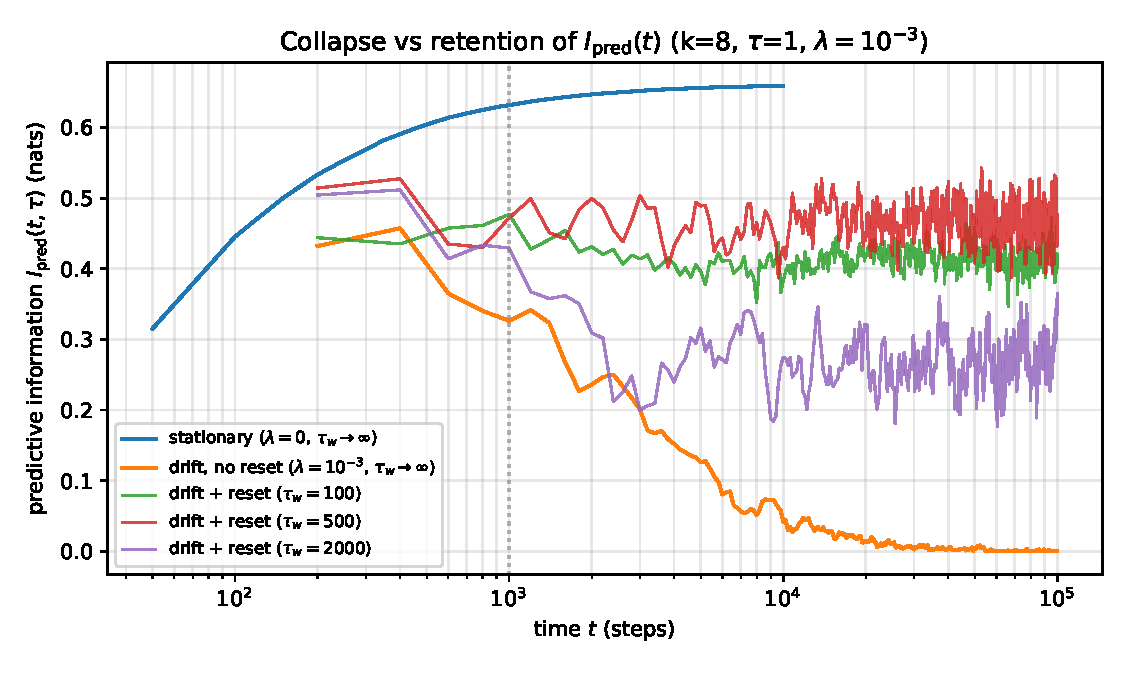
\includegraphics[width=0.85\linewidth]{figs/Fig1.pdf}\end{center}

 The diagnostically leading numerator. In the \textbf{stationary} regime (\(\lambda = 0\), \(\tau_w \to \infty\), \(T_{\text{sim}} = 10^4\)) \(I_{\text{pred}}\) \emph{is held} at \(\langle I_{\text{pred}}\rangle = 0.658 \pm 0.012\) nat --- the estimate keeps up with the environmental statics, \(\langle\nu^{\text{op}}\rangle = 0.006\). In the regime of \textbf{drift without reset} (\(\lambda = 10^{-3}\), \(\tau_w \to \infty\), \(T_{\text{sim}} = 10^5\)) \(I_{\text{pred}}\) \emph{collapses} to \(0.0007 \pm 0.0002\) nat --- a fall of \(\approx 940\) times relative to the stationary regime (ratio \(0.0011\)): the observer averaged \(\hat P\) over \(\sim 100\) independent past regimes and almost does not predict the current \(P(t)\). In the regime of \textbf{drift with reset} (\(\tau_w \in \{100, 500, 2000\}\), \(T_{\text{sim}} = 10^5\)) \(I_{\text{pred}}\) \emph{is held} at a positive level (\(0.41\), \(0.47\), \(0.27\) nat respectively) --- forgetting rescues prediction. This is the central result: the collapse of \(I_{\text{pred}}\) under memory accumulation and drift, removed by reset.



\emph{Fig. 2: optimal forgetting --- \(\langle I_{\text{pred}}\rangle\) as a function of \(\tau_w\)} 

\begin{center}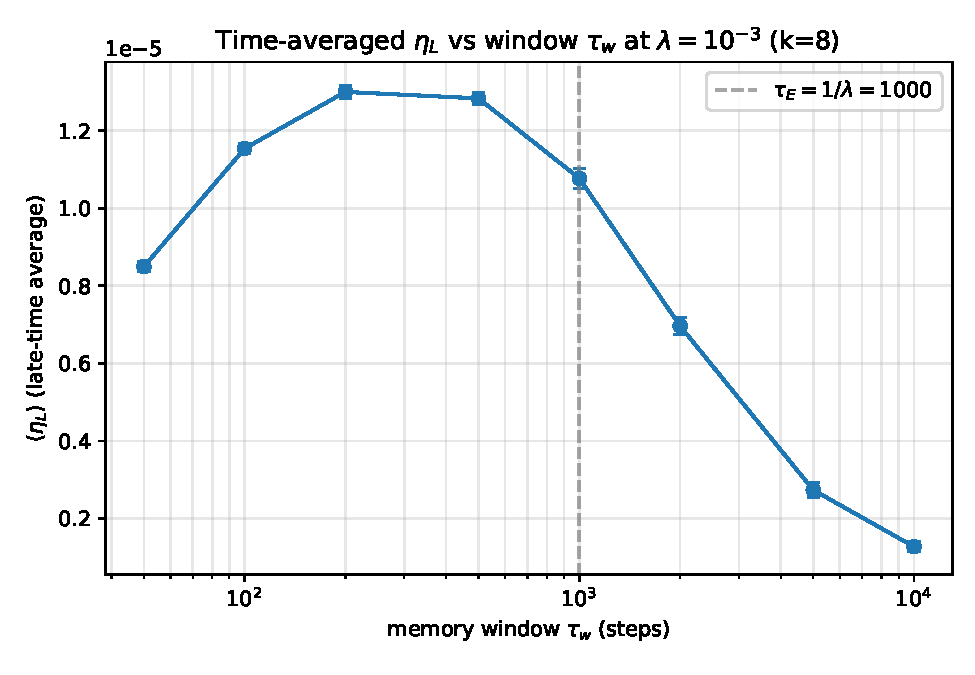
\includegraphics[width=0.85\linewidth]{figs/Fig2.pdf}\end{center}

 A dome-shaped curve (sweep \(\tau_w \in \{50, \dots, 10^4\}\), \(\lambda = 10^{-3}\), \(T_{\text{sim}} = 5\cdot 10^4\)) with a maximum \(\langle I_{\text{pred}}\rangle^* = 0.467 \pm 0.006\) nat at \(\tau_w^* \approx 200\) steps --- \emph{inside} the environmental correlation interval (\(\tau_w^* < \tau_E = 1000\)). Too short a window underestimates \(\hat P\) (few data), too long averages incompatible regimes; the optimum is a balance. This is an operational instantiation of (12) (\(\tau_{\text{reset}}^* < \tau_E\), \emph{forget at the pace of drift}) up to a logarithmic factor. (The secondary axis \(\langle\eta_v\rangle\) is structurally small, \(\sim 3\cdot 10^{-3}\), and its own optimum in \(\tau_w\) is shifted to \(\approx 100\) --- this is a diagnostic of ballast, not of prediction quality.)



\emph{Fig. 3: nostalgia \(\nu^{\text{op}}(t)\) and \(\nu^{\text{Still}}(t)\)} 

\begin{center}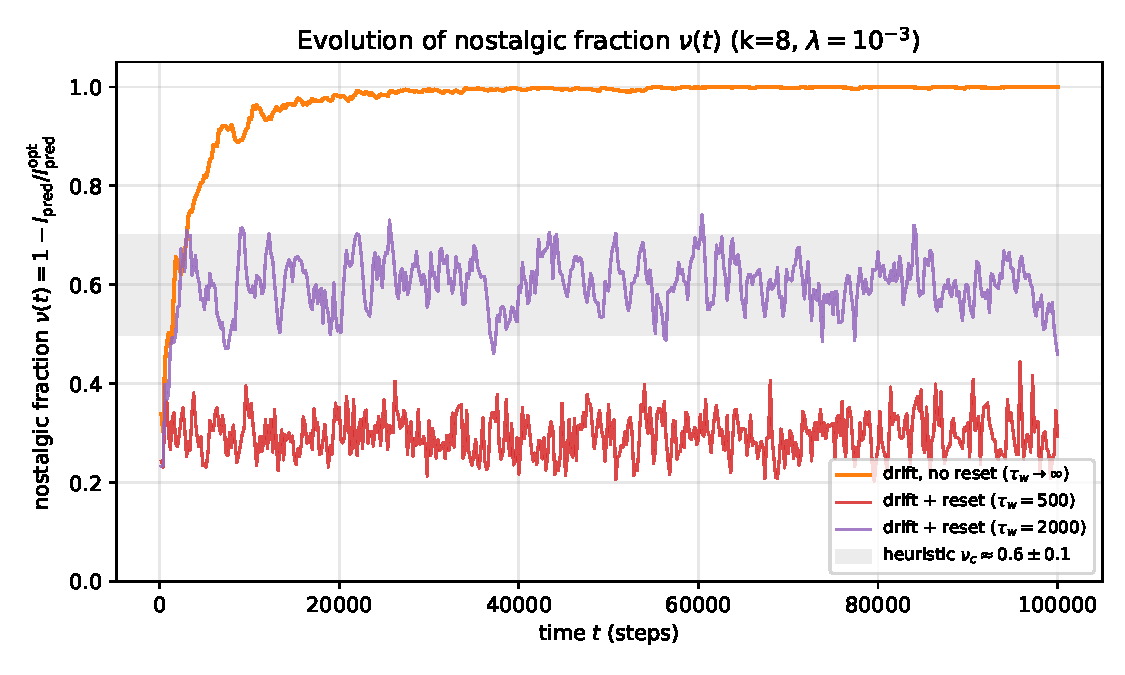
\includegraphics[width=0.85\linewidth]{figs/Fig3.pdf}\end{center}

 The operationally leading measure \(\nu^{\text{op}} = 1 - I_{\text{pred}}/I_{\text{opt}}\) (solid/dashed curves) \emph{distinguishes regimes}: in drift without reset \(\nu^{\text{op}}(t) \to 0.999\) --- almost complete nostalgia (a model accumulated over all past regimes is useless for the current one); in the regimes with reset \(\nu^{\text{op}}\) is bounded and depends on \(\tau_w\) (\(0.38\) at \(\tau_w = 100\); \(0.30\) at \(\tau_w = 500\); \(0.60\) at \(\tau_w = 2000\)) --- a minimum at the optimal window. The structural ballast \(\nu^{\text{Still}} = 1 - \eta_v\) in \emph{all} regimes with growing memory is \(\approx 0.997\)--\(1.000\) --- almost all held memory is ballast; it \textbf{does not distinguish} regimes (this is a structural property of a memory-accumulating learner, not a sign of collapse), and therefore the distinguishing scale is precisely \(\nu^{\text{op}}\). Validated limiting cases: under ideal learning \(I_{\text{pred}} \to I_{\text{opt}}\) (stationary, \(\nu^{\text{op}} \to 0\)); the capacity floor and the interior optimum in \(\tau_w\) are substantive precisely on the \(\nu^{\text{op}}\) scale.



Checks on all \(1.36 \cdot 10^5\) sampled points: \(\eta_v \in [0, 0.006]\) (boundedness is provided by finite-sample truncation § 3.1, not an empirically observed property). The substantive check of the floor (8a) goes on the shortfall scale \(\nu^{\text{op}} = \nu^{\text{theor}}\) (the oracle is available) --- see § 6.3; the ballast \(\nu^{\text{Still}} \to 1\) is trivial (§ 4.4) and is not a floor. The full parameters of the three regimes and the \(\tau_w\) grids, the simulation pseudocode (mutual information in the Markov model is computed exactly from the transition structure, without a sample estimator; the sample estimators Treves and Panzeri 1995, Kraskov et al.~2004 --- for data from real systems, § 3), the discussion of the dome-shaped dependence as a bias-variance trade-off, the divergence of \(C_v^{\text{static}}/C_v^{\text{predictive}}\) as a diagnostic signal of nostalgia --- Supplementary § S6.



\subsection{OU simulation: continuous drift of the logits}\label{ou-simulation-continuous-drift-of-the-logits}



The OU simulation at \(\sigma = 0.1\), \(\lambda = 10^{-3}\) (\(\sigma^2/\lambda = 10\), stationary variance \(\sigma^2/(2\lambda) = 5\), \(k = 8\), \(K = k(k-1) = 56\), \(T_{\text{sim}} = 2 \cdot 10^4\) steps, 50 realizations) is a numerical illustration of Lemma 2 in the canonical class of slow drift § 5.2 and of the central thesis of § 5.2 that \textbf{memory design decides}. On a \emph{single} OU trajectory of the logits (continuous drift without zeroing of the posterior, unlike the PSP surrogate § 6.1) two learners are compared:



\begin{itemize}

\tightlist

\item

  \textbf{Robbins--Monro} --- a decaying step \(\eta_t = c_0/\sqrt t\), \(c_0 = 3\) (asymptotically Bayes-optimal for \emph{stationary} regular models; Clarke and Barron 1990);

\item

  \textbf{constant step} \(s\) (operating point \(s = 0.3\), validated close to the optimum at \(\sigma = 0.1\)).

\end{itemize}



The slow-driving condition \(\lambda \tau_{\text{relax}} \ll 1\) holds with a large margin; OU-concentration (\(\sigma^2/\lambda \ll 1\)) does not hold, so the conjecture of Supplementary § S8.1 is not tested here. The common \(I_{\text{opt}} = 0.757 \pm 0.005\) nat (the predictability ceiling), \(I_{\text{mem}} = 268.7\) nat, \(N_{\text{obs}} = t\). The values are late-time averages (the last 50\%, \(\pm\) SEM over 50 realizations).



\emph{Why the leading measure is \(\nu^{\text{op}}\), not \(\eta_v\).} The memory capacity here is fixed (\(K\) parameters), and the figures report on the prediction shortfall \(\nu^{\text{op}}\) (normalization by the environmental optimum \(I_{\text{opt}}\)), not on \(\eta_v = I_{\text{pred}}/I_{\text{mem}}\). This is deliberate: \(\nu^{\text{op}}\) isolates the nontrivial floor of nostalgia (facet B, § 1) from the structural growth of the denominator \(I_{\text{mem}}\) (facet A), which would drive \(\eta_v \to 0\) regardless of tracking quality. The observed freezing vs.~tracking is an effect of the \emph{memory-update scheme}, not of the arithmetic of the denominator.



\emph{Fig. 4: nostalgia \(\nu^{\text{op}}(t)\) of both learners} 

\begin{center}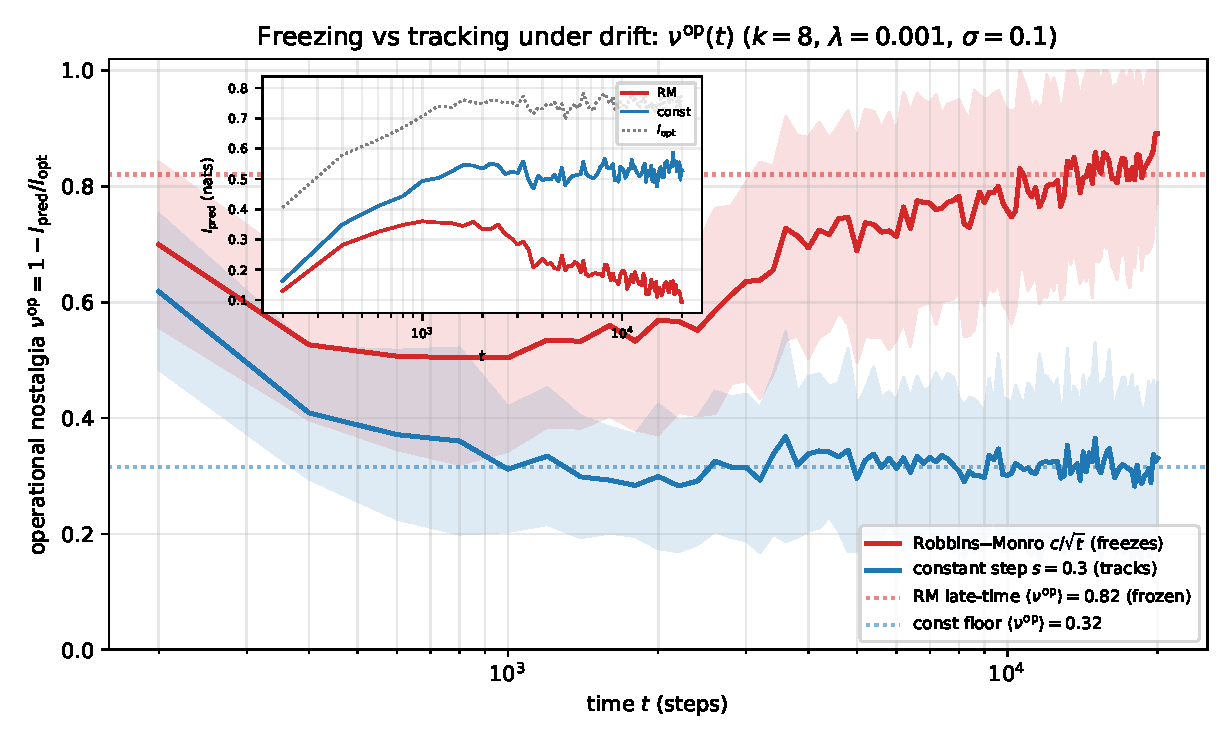
\includegraphics[width=0.85\linewidth]{figs/Fig4.pdf}\end{center}

 The load-bearing figure. The \textbf{Robbins--Monro learner freezes} under drift: its step decays faster than the environment drifts, the estimate stops tracking the moving \(\theta_v(t)\), and \(\nu^{\text{op}}(t)\) grows monotonically \(0.567 \to 0.747 \to 0.892\) (at \(t = 2200, 10200, 20000\)), to the late-time \(\langle\nu^{\text{op}}\rangle = 0.821 \pm 0.005\) (\(I_{\text{pred}} = 0.146\) nat, \(\theta_v\)-error \(15.4\)). The \textbf{constant-step learner tracks} the drift: \(\nu^{\text{op}}(t)\) holds at a \emph{floor} \(\approx 0.33\) (\(0.283 \to 0.305 \to 0.331\)), late-time \(\langle\nu^{\text{op}}\rangle = 0.316 \pm 0.003\) (\(I_{\text{pred}} = 0.529\) nat --- \(3.6\) times higher than RM). The inset shows \(I_{\text{pred}}(t)\) of both against \(I_{\text{opt}}\): RM collapses, the constant step holds below the optimum at a fixed lag price. This is a direct illustration of § 5.2: freezing vs.~tracking is determined by the \emph{memory-update scheme}, not by the environment alone.



\emph{Fig. 5: optimal step size} 

\begin{center}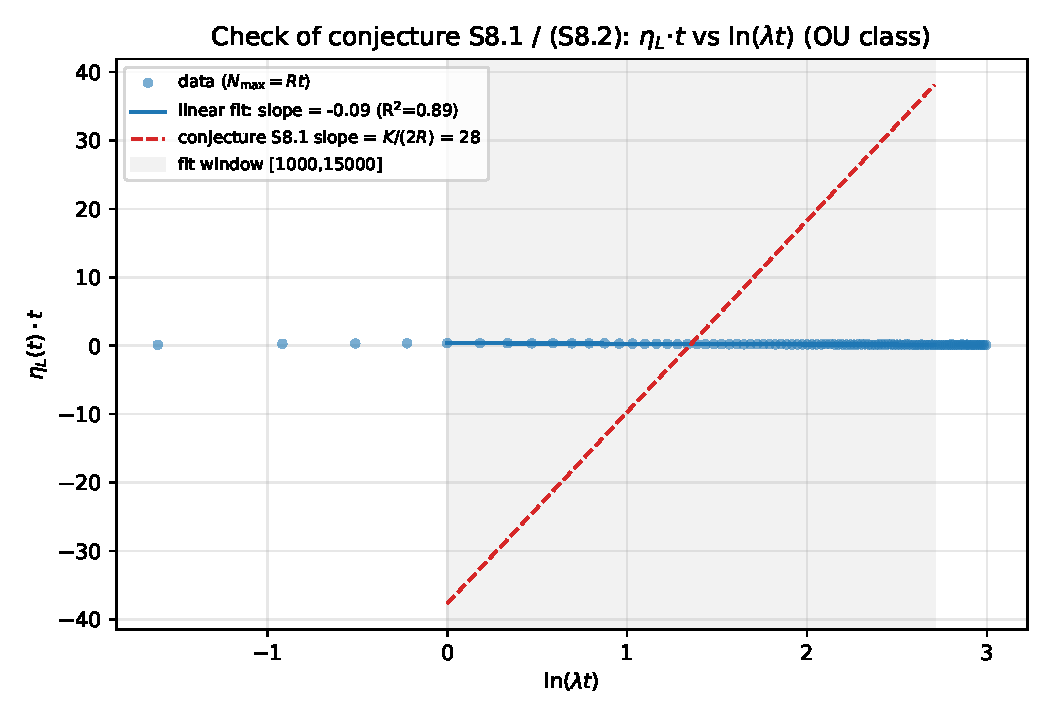
\includegraphics[width=0.85\linewidth]{figs/Fig5.pdf}\end{center}

 A sweep of the constant step size at \(\sigma = 0.1\) shows a non-monotone floor \(\langle\nu^{\text{op}}\rangle(s)\) with an \textbf{interior optimum} \(s^\star \approx 0.6\), \(\langle\nu^{\text{op}}\rangle = 0.290 \pm 0.004\): a small step (\(s = 0.02\): \(\nu^{\text{op}} = 0.861\)) gives lag (under-tracking), a large one (\(s = 1.0\): \(\nu^{\text{op}} = 0.339\)) --- the noise of overfitting; between them the optimum. All points of the sweep confidently beat the frozen Robbins--Monro (\(\langle\nu^{\text{op}}\rangle = 0.820\), dashed). A sweep in the drift strength \(\sigma\) confirms the separation: RM holds flat-high (frozen) at \(\nu^{\text{op}} \approx 0.82\)--\(0.86\) across the whole range \(\sigma \in [0.03, 0.4]\), whereas the constant step is \emph{responsive} to the drift (\(\nu^{\text{op}}\) from \(0.67\) at \(\sigma = 0.03\) to \(0.32\) at \(\sigma = 0.1\)). Substantively: the optimal learner forgets at the pace of drift; this links the result with continual learning --- the freezing of RM is the same mechanism as the catastrophic loss of plasticity under distribution shift (§ 8.4).



Checks on all \(5 \cdot 10^4\) sampled points of both learners: \(\eta_v \in [0, 0.008]\) (\(I_{\text{pred}} \le I_{\text{mem}}\) ensured by truncation § 3.1); the \textbf{substantive} check --- the shortfall \(\nu^{\text{op}} \in [0.010, 1.000] \subset [0,1]\) with zero cases of \(I_{\text{pred}} > I_{\text{opt}}\) (the numerator of \(\nu^{\text{op}}\) is \emph{not} truncated). The ballast measure \(\nu^{\text{Still}} = 1 - \eta_v \approx 1\) for both learners (memory of fixed size \(|M| = K\), but \(I_{\text{mem}} \gg I_{\text{pred}}\)): structurally \(\approx 1\), does not distinguish freezing from tracking --- it is precisely \(\nu^{\text{op}}\) that distinguishes, and that is why it is load-bearing.



The full parameters of both learners, the asymptotic Bayes-optimality of Robbins--Monro for the \emph{stationary} case and its breakdown under drift, the sweeps of \(\sigma\) and step size, the justification of the operating point \(s = 0.3\) --- Supplementary § S6. The full reproducibility parameters (seed \texttt{SEED\ =\ 20260524}, directories, library versions) --- Supplementary § S4.



\subsection{Conclusions from the simulations}\label{conclusions-from-the-simulations}



The two simulations --- PSP (§ 6.1) and OU (§ 6.2) --- perform \textbf{five concrete functions} with respect to the formal theory of §§ 4--5. They do \textbf{not} claim empirical validation on real biological systems (that is the task of the pre-registered protocols of § 8.6) and do \textbf{not} test the conjecture of Supplementary § S8.1 about the adiabatic asymptotics of \(L_{\text{excess}}\) (which requires the OU-concentration condition \(\sigma^2/\lambda \ll 1\), satisfied neither in PSP nor in OU § 6.2; the corresponding parametric scan --- Supplementary § S8.3).



\textbf{(1) Collapse of \(I_{\text{pred}}\), rescued by forgetting (the three regimes of § 5.1).} PSP reproduces all three regimes on the diagnostically leading numerator \(I_{\text{pred}}\): \emph{holding} in the stationary case (\(0.658\) nat), \emph{collapse} under drift without reset (\(0.0007\) nat --- a fall by a factor of \(\approx 940\)) and \emph{holding under reset} (\(0.27\)--\(0.47\) nat). OU reproduces the same fork on continuous drift through \emph{learner design}: Robbins--Monro collapses (freezes, \(I_{\text{pred}} = 0.146\) nat), the constant step holds (\(0.529\) nat). The central result --- the collapse of \(I_{\text{pred}}\) under memory accumulation and drift, removed by forgetting/reset --- is \emph{confirmed} in both parameterizations.



\textbf{(2) Memory design decides (§ 5.2).} The OU simulation directly instantiates the thesis: the Robbins--Monro learner (a decaying step, Bayes-optimal for the stationary case) \textbf{freezes} under drift --- \(\nu^{\text{op}}\) grows \(0.567 \to 0.892\); the constant step \textbf{tracks} to the floor \(\nu^{\text{op}} \approx 0.32\). The \(\sigma\)-sweep confirms this: RM is flat-high (\(\nu^{\text{op}} \approx 0.82\)--\(0.86\), insensitive to drift --- frozen), the constant step is responsive. There exists an \textbf{optimal step} \(s^\star \approx 0.6\) (\(\nu^{\text{op}} = 0.290\)), beating the frozen RM (\(0.820\)). The meaning --- to forget at the pace of the drift: neither slower (freezing) nor faster (noise overfitting).



\textbf{(3) Lemma 2: the floor of nostalgia is satisfied.} PSP with drift without reset gives \(\nu^{\text{op}}_\infty \to 0.999\) on the operationally leading scale of the prediction shortfall --- this is precisely the direct check of the floor (8a): at an almost zero rate of update \(\dot M_{\text{refresh}} \to 0\) the fraction \(c = \dot M_{\text{refresh}}\,\tau_E/|M_{\le t}| \to 0\), and \(\nu^{\text{op}} \ge 1 - c \to 1\) (observed \(0.999\)). The structural ballast \(\nu^{\text{Still}} \to 1.000\) on its own scale is trivial and does \emph{not} test the regime (§ 4.4). In OU the constant step holds \(\nu^{\text{op}}\) below unity precisely because it updates memory at the pace of the drift (the fraction \(c\) is large) --- consistent with the fact that the floor \(1-c\) of the Lemma is the lower, the higher the refresh rate relative to \(\tau_E\). A quantitative check of the bound \(1-c\) as a \emph{pointwise} prediction on a concrete system with a controlled \(\tau_E\) is deferred to the pre-registered protocol on \emph{E. coli} (§ 8.6).



\textbf{(4) The existence of \(\nu_c\) and of optimal forgetting (§§ 5.3, (12)).} The dome-shaped curve \(\langle I_{\text{pred}} \rangle(\tau_w)\) (Fig. 2) with a maximum \(\langle I_{\text{pred}}\rangle^* = 0.467\) nat at \(\tau_w^* \approx 200 < \tau_E = 1000\) is an operational instantiation of (12) (\(\tau_{\text{reset}}^* < \tau_E\)) up to a logarithmic factor; the existence of an optimum as a function of the structural parameters (\(\tau_E\), \(\dot M_{\text{refresh}}\), \(|M_{\le t}|\)) is a measurable effect on the synthetic benchmark, not a postulate. The continuous analogue is the optimal step \(s^\star \approx 0.6\) (Fig. 5). This gives an \textbf{operational handle} for the pre-registered prediction P.1 (§ 8.6): the divergence \(C_v^{\text{static}}/C_v^{\text{predictive}}\) as a diagnostic signal of the regime threshold \(\nu_c\) on the prediction-shortfall scale (the open problem of a quantitative formula --- § 8.5).



\textbf{(5) The bridge to continual learning (§ 8.4).} The freezing of Robbins--Monro under drift is structurally equivalent to the catastrophic loss of plasticity of an online learner under distribution shift; the constant step --- to a regime of continual adaptation. An important caveat: the naive ML form of the prediction (a monotone growth of \(\nu^{\text{op}}\) with the strength of drift for \emph{any} learner) is refuted by the fact that the constant step does \emph{not} follow it --- robustness to drift is a property of the memory design, not an inevitability; the load-bearing falsifier of the transfer of Lemma 2 remains biological (\emph{E. coli}, § 8.6).



\textbf{What the simulations have validated.} On all sampled points: \(\eta_v \in [0,1]\) (boundedness ensured by the finite-sample truncation \(I_{\text{pred}} \gets \min(I_{\text{pred}}, I_{\text{mem}})\) § 3.1 --- an estimator guard, not a confirmation of the bound); the \textbf{substantive} check --- \(\nu^{\text{op}} \in [0,1]\) with zero cases of \(I_{\text{pred}} > I_{\text{opt}}\) on \(1.36 \cdot 10^5\) points of PSP and \(5 \cdot 10^4\) points of OU (the numerator of \(\nu^{\text{op}}\) is not truncated). The limiting cases are reproduced: ideal learning \(I_{\text{pred}} \to I_{\text{opt}}\) (\(\nu^{\text{op}} \to 0\)) in the stationary case; full collapse (\(\nu^{\text{op}} \to 1\)) under drift without update; the interior optimum of forgetting. The ballast floor of Lemma 2 is satisfied (item 3).



\textbf{What the simulations do \emph{not} do.} (a) They do not validate the theory on real biological systems --- that is the task of § 8.6 P.2 (\emph{E. coli} chemotaxis). (b) They do not prove the conjecture of Supplementary § S8.1 about the asymptotics \((K/2)\ln(\lambda t)\) for \(L_{\text{excess}}\) --- this needs the adiabatic OU regime \(\sigma^2/\lambda \ll 1\), tested separately in Supplementary § S8.3 (status: an open conjecture, not a theorem). (c) They do not close the transfer of Lemma 2 to non-OU classes (multi-scale drift, fractional OU) --- Remark 4 § S5.1 restricts the rigorous proof to the OU class.



\emph{A caveat on the structure of \(\eta_v\).} \(\eta_v \sim 10^{-3}\) is structurally small in all regimes with a growing memory (facet A, § 1) --- this is not a signal of quality (``high''/``catastrophically low'') but a property of accumulation; the regimes are distinguished by \(\nu^{\text{op}}\), while \(\nu^{\text{Still}}\) carries the thermodynamic bound.



Summary: the simulations confirm the qualitative structure of the theory and provide an operational handle for the pre-registered predictions (P.1, P.2 § 8.6), remaining within the domain of applicability through the explicit satisfaction of \((*)\) and slow-driving.



\section{Connection with active inference and unsupervised learning}\label{connection-with-active-inference-and-unsupervised-learning}



The connection between \(\eta_v\) and Friston's free energy principle (Friston 2010; Friston et al.~2017a) is formulated in (Andriishin 2026, § 4.4): the requirement of self-payment turns the FEP into a discriminative criterion, and \(\eta_v\) operationally closes the gap between the general formalism and the requirement that the energy belong to the modeling loop. In the non-stationary regime the Pearl/Friston-blanket demarcation (Bruineberg et al.~2018; Bruineberg et al.~2022) is preserved: the correspondence between \(\eta_v\) and EFE makes sense only for systems that pass the self-payment test (\(S=1\), § 2.7); self-payment here is an \emph{alternative} ontology, not a constitution of the Friston blanket (cf.~Andriishin 2026, § 4.4: the question shifts from ``does a Friston blanket exist'' to ``is the holding of the model paid for''). For systems without self-payment (\(S=0\)) there is no correspondence.



In the non-stationary regime \(\eta_v(t)\) structurally corresponds to the epistemic component of the expected free energy \(G[\pi]\) (Friston et al.~2017a; Parr et al.~2022) in the slow-driving limit. \textbf{This correspondence is fixed as a \emph{heuristic correspondence} (Supplementary § S7.1), not as a proven inequality}; the conjecture about an equivalent inequality (Supplementary § S7.2) is an open problem. A categorical caveat: \(I_q(s'; o' \mid \pi)\), the epistemic value of AIF, and \(I(X_t; X_{t+\tau} \mid \hat P(t))\) of the present work are different MI objects (policy-contextual versus observational); the bridge through the sufficiency of \(\hat P(t)\) gives a lower bound on the epistemic value (equivalently, an upper bound on \(I_{\text{pred}}\), Supplementary § S7.3), not an equality. The correspondence is \emph{partial, in the epistemic component}, not an equivalence; the pragmatic component through the preference \(C\) remains outside the thermodynamic scale. A \emph{hypothetical} active-inference algorithm with an extended objective function including \(\dot E_{\text{store}}\) in the pragmatic part of the preferences would balance the reduction of nostalgia against the exploitation of the model with the optimum (12); existing AIF implementations (Friston et al.~2017a; Parr et al.~2022; Friston et al.~2021) optimize \(G[\pi]\), not \(\eta_v(t)\). The connection with intrinsic motivation (Schmidhuber 1991; Friston et al.~2017b) and meta-learning (Finn et al.~2017): in a non-stationary environment, exploration is \emph{informationally} necessary for \(\eta_v > 0\) (without memory update \(I_{\text{pred}} \to 0\); thermodynamics enters through the cost of holding, not as the source of the necessity itself).



\emph{The informational rejuvenation metric.} The ratio of the rates of update and of memory growth



\begin{equation}\rho(t) = \frac{\dot{M}_{\text{refresh}}(t)}{\dot{M}_{\text{grow}}(t)} \tag{13}\end{equation}



--- a diagnostic independent of a direct measurement of \(\nu(t)\): \(\rho \gg 1\) --- the update outruns the growth, nostalgia is low; \(\rho \ll 1\) --- the archival layer becomes nostalgic. The empirical calibration of \(\rho_c\) is a separate study.



The full formal correspondence between \(\eta_v\) and EFE with unit conversion through \(\beta_v = 1/(k_B T)\), the heuristic correspondence for the increment \(\Delta G^{\text{epist}}\) against \(\Delta I_{\text{pred}}\), the conjecture about an equivalent inequality, the categorical caveat \(I_q(s'; o') \ne I(X_t; X_{t+\tau})\), the context of sophisticated inference (Friston et al.~2021), the rebuttal of Andrews (2021) / Williams (2020) through a cross-reference to (Andriishin 2026, § S4.4a), and an analysis of the informational-rejuvenation metric \(\rho(t)\) (its refresh/grow poles and bacterial instantiation) --- Supplementary § S7.



\section{Discussion, open questions and conclusion}\label{discussion-open-questions-and-conclusion}



\subsection{Summary}\label{summary}



The work methodologically extends (Andriishin 2026) to the non-stationary regime: three structural results, a methodological toolkit, one open quantitative conjecture.



\textbf{Three structural results.}



\begin{enumerate}

\def\labelenumi{\arabic{enumi}.}

\item

  \emph{The price of a growing memory (Lemma 1 and the thermodynamic floor).} The predictive efficiency \(\eta_v(t)\) is measured on a \emph{growing} denominator --- the full held memory, which accumulates as learning proceeds (§ 2.1, § 5.1). The thermodynamic price of this holding is carried into a separate, cumulative form of the Still bound: over the whole history the system dissipates no less than the ``cost'' of the held non-predictive ballast (§ 2.2). Lemma 1 gives the minimal power required to hold a single bit against thermodynamic erosion (§ 2.3).

\item

  \emph{Nostalgia on a growing memory (Lemma 2).} The predictive information is generalized to the full --- current plus archival --- memory (§ 3), and nostalgia itself is separated into two lines: the operationally leading \emph{prediction shortfall} (in a theoretical and in a measurable version) and the secondary structural--thermodynamic \emph{ballast}, which carries the Still bound (§ 4.1). Lemma 2 gives a \emph{conditional} floor: under slow Gaussian drift (the OU class, § 5.2) and a finite update rate the prediction shortfall asymptotically does not fall below the computable bound \(1 - \kappa c\) (\(\kappa = 1 + o(1)\) empirically, § 4.4), while the efficiency \(\eta_v(t)\) passes through three regimes (§ 5.1).

\item

  \emph{The threshold and the optimal reset.} A regime threshold \(\nu_c\) is singled out, separating adaptive memory from nostalgic collapse (§ 5.3), together with the optimal interval of periodic memory reset \(\tau_{\text{reset}}^*\), consonant with the timescale of epigenetic reprogramming (§ 5.3).

\end{enumerate}



\emph{The methodological toolkit:} the distinction between the theoretical and the measurable prediction shortfall (§ 4.1); the static versus the predictive operationalization of the self-model capacity as a diagnostic of nostalgia (§ 4.3); the discipline of the protocol against ad hoc rescues (§ 5.2, Supplementary § S5.2); and two pre-registered protocols (§ 8.6).



\textbf{The quantitative conjecture is carried into Supplementary § S8.} A separate conjecture about the adiabatic asymptotics of the accumulated predictive loss is an \emph{unconfirmed secondary superstructure}, not a result of the work: the numerical scan supports its functional form but does not distinguish a slow convergence to the limit from a plateau below it, and so we do not claim it as an attainable law. The load-bearing core of the work does not depend on it; the technical reconciliation of the coefficients --- § S8.3.



\emph{The strongest objection and the reply to it.} Let us name the sharpest objection directly: the adiabatic asymptotics carried into the supplementary did not pass independent numerical checks (§ 6, § 8.5) and remains an unconfirmed conjecture, not a result. The reply: the load-bearing core of the work does \emph{not} depend on it --- Lemmas 1 and 2, the computable bound on the prediction shortfall, the separation of ballast and shortfall, the self-payment criterion and the methodological protocol are proved or formulated independently of this asymptotics. Its refutation touches none of the core claims.



The numerical illustrations (§ 6) demonstrate Lemma 2 and the three regimes of \(\eta_v(t)\); the efficiency \(\eta_v(t)\) corresponds to the epistemic component of the expected free energy of active inference (§ 7), where the informational rejuvenation metric \(\rho(t)\) is also introduced.



\textbf{Structural results and context-dependent specifications.} \emph{Structural results} (general statements independent of the choice of parametric class): self-payment in the non-stationary regime (§ 2.7); the stationary result of article \#1 as a particular case; \(\eta_v(t) \in [0, 1]\) by DPI for the conceptual numerator (§ 2.1); the cumulative Still bound ((2-cum), § 2.2) and Lemma 1; Lemma 2; the existence of \(\nu_c^{\text{theor}}\) on the prediction-shortfall scale (with a working assumption of stability under a change of normalization, § 4.1); the separation of nostalgia-ballast \(\nu\) and the prediction shortfall \(\nu^{\text{theor}}\)/\(\nu^{\text{op}}\); the protocol of § 5.2 / Supplementary § S5.2. \emph{Context-dependent specifications} (dependent on the concrete parametric class or operational choice): the drift class (OU/PSP --- piecewise-stationary); the numerical estimate of \(\nu_c^{\text{op}}\); the choice of the window \(\tau\); the operationalizations of the self-model capacity \(C_v\) (article \#1); the open quantitative conjecture of Supplementary § S8.



\subsection{What is NOT done in this work}\label{what-is-not-done-in-this-work}



The work is limited to theory. Beyond it lie --- (i) the empirical calibration of \(\eta_v(t), \nu(t), \rho(t)\) on concrete biospheres, cities, LLMs (this requires an operationalization of \(E_{\text{store}}, E_{\text{grow}}\) for each class); (ii) a full theory of cognitive systems as an \(\eta_v\)-problem (psychological memory, forgetting, everyday nostalgia as phenomenal states of a subject --- a categorically distinct referent from the informational nostalgia of the present work); (iii) the philosophical consequences of the distinction between the current and the archival memory layers (semantic versus episodic memory, the role of forgetting in identity).



\subsection{LLM-corp as a cross-domain illustration (a boundary case)}\label{llm-corp-as-a-cross-domain-illustration-a-boundary-case}



The class of large language models trained on a static corpus and exploited in a drifting environment figures as a \emph{cross-domain illustration} of the applicability of the formalism to non-biological systems, not as an independent empirical application (the central prediction of the work is \emph{E. coli} chemotaxis, § 8.6 P.2).



\emph{The boundary and self-payment} (§ 2.7). In a strict stateless LLM-as-agent the self-payment loop is structurally open: \(\dot E_{\text{store}}\) is paid for by an external data center, and \(\eta_v\) is undefined. By the escalating boundaries of paper \#1 (Andriishin 2026, § 3.4 + Supplementary § S3.4), \(\eta_v(t)\) is defined only starting from the \(B_4\)-boundary (the corporation as a legal entity): the current layer \(M_t\) is the KV-cache plus the operational state of the corporation, the archival \(M_{\lt t}\) the weights plus the corporate corpus, the environment \(X_E\) the statistics of queries, drifting by vocabulary (Lazaridou et al.~2021; Dhingra et al.~2022). This is an \emph{honest downgrade in status}: the formalism itself takes open configurations out of the domain of applicability rather than being stretched onto them.



\emph{A two-layer prediction.} For the archival layer of an overtrained LLM without continual pre-training (\(\dot{M}_{\text{refresh}}^{\lt t} \approx 0\), \(c \approx 0\)) Lemma 2 gives \(\liminf \nu_{\lt t}(t) \ge 1\) --- the weights become stale as language drifts, which qualitatively is a monotone growth of perplexity on texts after the cutoff moment --- a \textbf{known observation} (Lazaridou et al.~2021; Dhingra et al.~2022), not an original prediction. For the current layer of long-context models, \(c\) for the \(M_t\)-layer \(\gg 1\), and Lemma 2 \emph{is not applicable to it} (a sliding-window regime, an explicit self-restriction through \((*)\)).



\emph{Refresh channels and an open question.} In-context learning updates only \(M_t\); continual pre-training and RAG with an updatable index (Lewis et al.~2020; Borgeaud et al.~2022; Khandelwal et al.~2020; Izacard et al.~2023) are a refresh channel for \(M_{\lt t}\) (a comparison of perplexity with/without an updatable RAG is an operational prediction). An open question: does \emph{implicit in-context adaptation} (induction heads --- Olsson et al.~2022; ICL of functional classes --- Garg et al.~2022; Bricken et al.~2023) induce an implicit update of the archival layer; if not --- \(\nu_{\lt t} \to 1\) remains for all long-context LLMs without RAG.



\subsection{Connection with continual learning}\label{connection-with-continual-learning}



Catastrophic forgetting (McCloskey and Cohen 1989; Goodfellow et al.~2014; Kirkpatrick et al.~2017; Lopez-Paz and Ranzato 2017; Riemer et al.~2019; Parisi et al.~2019) has a natural interpretation within the framework of the theory; a parallel apparatus is the stochastic thermodynamics of learning (Goldt and Seifert 2017). Concept drift (Gama et al.~2014; Bifet and Gavaldà 2007) is unified through the bridge (8): drift detectors fire when \(\nu(t) > \nu_c\). Catastrophic forgetting is a \emph{failure} of holding predictive memory (overwriting without allocating \(E_{\text{grow}}\)), not a deliberate reduction of \(\nu(t)\). The methods of combating it map onto the balance differently: progressive networks and replay buffers --- an investment in \(E_{\text{grow}}\) (growth of the substrate), whereas EWC (Kirkpatrick et al.~2017) is a regularization \emph{protecting} predictive weights from overwriting (a reduction of \(\nu\) without a growth of capacity).



Nostalgia and catastrophic forgetting are two poles of the balance of \(\dot{E}_{\text{store}}\) and \(\dot{E}_{\text{grow}}\): nostalgia is an \emph{excess} of non-predictive memory, forgetting a \emph{deficit} of prematurely erased memory. The optimum is (12). As \(\lambda \to 0\) nostalgia reduces to \emph{overfitting}.



\emph{Contrast with a renaming --- a comparison with ML precedents.} To the objection ``nostalgia is a renaming of concept drift + forgetting + dynamic regret'': the theory contains constructions structurally close to known ML results, but operationally and in scale distinct from them.



\emph{The protocol worked on the authors themselves.} The point of the protocol (§ 5.2) prohibiting a post-hoc redefinition of the object of measurement is a real constraint, not a ritual: the temptation to replace the operationally measurable \(I_{\text{pred}}\) with the counterfactual \(L_{\text{excess}}\) (under which the asymptotics holds), while keeping the name of the theory, is prohibited by the protocol --- \(L_{\text{excess}}\) is carried into § S8 as a secondary metric, the asymptotics is marked as an open conjecture (details --- § 8.1).



\textbf{(a) Lemma 2 versus Besbes--Gur--Zeevi 2015 (dynamic regret).} (Besbes et al.~2015) (Theorem 2) give for a sliding-window learner a regret \(R_T = O(V_T^{1/3} T^{2/3})\); the parallelism is obvious. The difference: this is a \emph{sample-level upper bound} on regret for \(V_T = o(T)\), whereas Lemma 2 is an \emph{informational} lower bound on the prediction shortfall \(\nu^{\text{theor}}(t)\) (the unattainable fraction of the predictable future) in the OU class of § 5.2, with a separate thermodynamic floor of holding this fraction through the cumulative Still bound ((2-cum), (8)), that is, a lower bound on a measure that sample-level regret does not reflect.



\textbf{(b) \(\tau_{\text{reset}}^*\) versus the optimal length of the sliding window (Hazan and Seshadhri 2009; Karnin and Anava 2016).} There \(\tau_{\text{reset}}\) is an \emph{algorithmic} restart parameter without a thermodynamic interpretation; in (12) it is a \emph{physical} interval of periodic memory erasure, optimizing \(\eta_v\) through the trade-off of \(\dot E_{\text{store}}\) against \(\dot E_{\text{grow}}\) (the biological instantiation is the generation time of epigenetic reprogramming, § 4.4).



\textbf{(c) \(\nu_c\) versus phase transitions in ML.} \(\nu_c \in (0,1)\) (11) is \emph{not} equivalent to grokking (Power et al.~2022) (a reorganization of weights at a fixed environment) or double descent (Belkin et al.~2019) (generalization versus capacity at a fixed task): \(\nu_c\) is a transition in \emph{memory composition} under a drifting environment and a fixed architecture; the connection is non-trivial (§ 8.5).



\textbf{(d) The thermodynamic scale \(k_B T \ln 2\) is absent from the ML literature.} Nostalgia as an energetic quantity is not defined there; \(\dot{E}_{\text{store}}^{\text{nostalg}} \ge k_B T \ln 2 / \tau_{1/2}\) is a bridge between the informational measure \(\nu\) and the physical budget, unliftable within ML formalisms (Still et al.~2012; Gama et al.~2014; Kirkpatrick et al.~2017). In the biological paradigm case, by contrast, the energetics of adaptation is an established fact: the price of accuracy and rate of sensory adaptation has been quantitatively described for \emph{E. coli} chemotaxis (Lan et al.~2012; Mehta and Schwab 2012). The contribution of the present work here is not the first introduction of energetics into chemotaxis, but a \emph{non-stationary lower bound on the accumulation of nostalgia} --- on the flow of holding the stale fraction of memory over time, not on a single adaptation.



\emph{An operational handle on \(c\) for ML.} For SGD with a rate \(\eta_t\) on \(N\) parameters at a permutation frequency \(\rho_p\) (\(\tau_E = 1/\rho_p\)) the update rate \(\dot M_{\text{refresh}} \approx \eta_t N\), \(|M_{\le t}| \approx N\), whence \(c \approx \eta_t/\rho_p\) (order-of-magnitude; the exact value is calibrated empirically). Fast drift (large \(\rho_p\)) gives a small \(c\) and high nostalgia \(\nu \to 1-c\); slow --- a large \(c\), a sliding-window regime where Lemma 2 is not applicable. A caveat about the classical Permuted MNIST (Goodfellow et al.~2014): there each permutation is fine-tuned to convergence, that is, the change is \emph{rare} (small \(\rho_p\), large \(c\)); and its metric is the drop of accuracy on past tasks, not \(\nu^{\text{op}}\), which cannot be identified.



\emph{The ML form of the prediction.} Naively: for a trainable MLP without EWC/replay the nostalgic fraction grows with \(\rho_p\), where \(\nu^{\text{op}}\) is proxied by the ablation fraction --- the fraction of hidden units whose zeroing does \emph{not} raise the current-task loss. This is only a \emph{proxy} of the canonical \(\nu^{\text{op}} = 1 - I_{\text{pred}}/\hat E\) (§ 4.1), not an identity, and requires a control of learnedness.



\emph{A reproducible benchmark and an honest negative result} (\texttt{simulations/permuted\_mnist/}: \texttt{sklearn.load\_digits} \(8\times8\), MLP \(64\to32\to10\), online SGD). The naive form \textbf{does not survive}: the naive proxy \(\nu^{\text{op}} \approx 1 - \text{learnedness}\) \textbf{conflates nostalgia with under-learning} --- under fast drift the network mechanically fails to learn the task (accuracy \(\to\) chance), and the proxy grows irrespective of nostalgia. After an accuracy gate and a definition of \emph{true} nostalgia (a unit is useless now \textbf{and} was useful on a recent past permutation) the effect \textbf{disappears and reverses} (\(\nu^{\text{op}}_{\text{true}}\) anti-correlates with \(\rho_p\); Spearman \(= -1.0\) on four seed-averaged points --- only the sign is meaningful (the per-run distributions of adjacent \(\rho_p\) overlap); the full numbers and spread in the benchmark's README). The reason: SGD is a high-refresh learner, permanently in the large-\(c\) regime (sliding window), so the small MLP does \textbf{not} instantiate the law \(c \to \nu\) cleanly; the leading driver here is re-specialization under a long dwell.



Substantively this is the \textbf{third honest negative test} of the article --- after the check of the PSP bound (§ 6.1) and of the OU class for the adiabatic asymptotics (§ 6.2). The methodological protocol of § 5.2 (the priority of falsifiability over confirmation) worked here too: without a control of learnedness the confound-driven ``confirmation'' would have been kept as valid; the control held it back from that. The load-bearing falsifier of Lemma 2 remains \textbf{biological} --- bacterial \emph{E. coli} chemotaxis (§ 8.6); the naive ML form is refuted by its own benchmark and is not offered as a confirmation.



\emph{Class-restriction and no-free-lunch.} Wolpert's no-free-lunch (Wolpert 1996) gives a fundamental justification for the narrowing of the class (§ 5.2): a universal theory of non-stationary learnability without an a priori restriction of the class is impossible; class slow-driving is one of the sufficient narrowings (NFL justifies that \emph{some} narrowing is necessary, not this one specifically), chosen as canonical and biologically motivated.



\subsection{Open problems}\label{open-problems}



\emph{Three connected open problems.} (i) the transfer of the floor \(\liminf\nu^{\text{theor}} \ge 1-c\) beyond the OU class; (ii) the status of the adiabatic asymptotics \((K/2)\ln(\lambda t)\); (iii) the behavior under superlinear memory growth \(|M_{\le t}| \propto t^\alpha\). A related conceptual question is also open: does the thermodynamic price of holding (the ballast \(\nu^{\text{Still}}\), the load-bearing bound) \emph{track} the regime collapse (the prediction shortfall \(\nu^{\text{op}} \to 1\)), or does it stand apart from it --- that is, is the apparent juxtaposition of the structural ballast and the regime-distinguishing shortfall essential.



\emph{The conjecture about the adiabatic asymptotics (Supplementary § S8).} The conjecture of Supplementary § S8.1 about the asymptotics of the cumulative excess-loss \(L_{\text{excess}}(t) \sim (K/2)\ln(\lambda t)\) in the OU class at \(\sigma^2/\lambda \ll 1\) remains \emph{open and unconfirmed}. The analytical value \(K/2\) is derived as an identity of the limit \(\epsilon_{\text{track}} \to 0\), and the numerical scan of Supplementary § S8.3 supports the functional form (\(R^2 \ge 0.9995\) in the fit \(A t + B\ln(\lambda t) + C\)), but the fitted \(B/(K/2)\) grows monotonically (\(0.54 \to 0.85\) as \(\sigma^2/\lambda\) goes from \(10^{-1}\) to \(10^{-3}\)), without reaching unity. Such behavior is consistent rather with the limit being structurally \emph{unattainable} (the adiabatic logarithm is realized only transiently, after which \(L_{\text{excess}}\) reaches a plateau) than with an insufficiency of the scan points. We therefore do \emph{not} claim the asymptotics as an attainable law; all the more open is its transfer to the operationally measurable \(\eta_v(t)\) (\(\dot\eta_v^{\text{excess}}\)).



\emph{The extension of Lemma 2 to a fast-growing memory.} The current Lemma 2 relies on the boundedness of \(|M_{\le t}|\) through the constant \(c\) from \((*)\). At \(|M_{\le t}| \propto t^\alpha\) (\(\alpha \ge 1\)) the condition \(c \lt 1\) becomes trivially satisfiable, but the qualitative picture of nostalgia changes: with a sufficiently fast growth of capacity the nostalgic fraction may remain a finite fraction. A formal extension of Lemma 2 to this regime is an open problem of non-stationary Bayesian models.



\emph{Connection with fluctuation theorems.} The theorems of Crooks (Crooks 1999) and Jarzynski (Jarzynski 1997); the generalization with feedback control (Sagawa and Ueda 2010) gives a bridge to the decomposition (1) through the measurement channel. An application to the balance of \(E_{\text{store}}, E_{\text{grow}}, E_{\text{actual}}^{\text{curr}}\) may give finer inequalities than the Landauer bound.



\emph{The operationalization of \(E_{\text{store}}\) for cultural and biospheric memory.} \(\tau_{1/2}\) is quantitatively different (epigenetics, genome, synapses); in cultural systems the substrate is ambiguous (a book, a digital archive, a neural network) --- a separate study.



\emph{Refinement of the regime threshold \(\nu_c\).} The existence of a strict transition with universal critical exponents and a numerical estimate for the paradigm classes is an open question. Here also --- the \emph{stability of \(\nu_c\) under a change of normalization} (§ 4.1): a rigorous theorem on the monotonicity of the regime threshold under the DPI inequality \(\nu^{\text{op}} \le \nu^{\text{theor}}\), justifying the transition from \(\nu_c^{\text{theor}}\) to \(\nu_c^{\text{op}}\) in the pre-registered protocol of § 8.6 (P. 1).



\emph{Analytical closure of per-bit-uniformity.} The per-bit-uniformity assumption of Remark 5 (additivity of MI over independently updated bits with a constant \(1+o(1)\), § 4.4) is in the present work checked \emph{numerically} (§ 6.2) and relies on the degeneracy of the inter-coordinate coupling \(\kappa \to 0\) at the parameters of the OU scan of § 6.2 (independence of the logits, Supplementary § S2.2/§ S2.7); it has no general analytical proof. At a nonzero coupling \(\kappa > 0\) the additivity constant deviates from \(1\), and the transition from the bit-fraction \(c\) to the information ratio \(\nu^{\text{theor}} \ge 1 - c\) requires a separate estimate. An explicit bound on \(|1 - \text{const}|\) as a function of \(\kappa\) (an analytical closure beyond the degenerate regime of § 6.2) is an open problem.



\emph{Regularity of the softmax parameterization.} A full proof of the transfer of the OU decorrelation to the nonlinear softmax parameterization of the transition matrix (Remark 6 § 4.4) is a technical extension through Lipschitz continuity in total variation on the part of the OU trajectory bounded with probability \(1-\delta\); it gives the convergence \(\nu(t) \to 1 - c\) in the concrete OU parameterization of § 6.2 / Supplementary § S6.3 beyond the illustrative \(\liminf\)-inequality (8a).



\subsection{Empirical predictions}\label{empirical-predictions}



The theory formulates two core-empirical predictions (P. 1, P. 2).



\emph{Prediction 1: the existence of a regime threshold \(\nu_c^{\text{op}} \in (0, 1)\).} In adaptive non-stationary systems with a finite rate of memory update there must exist a critical level of nostalgia \(\nu_c^{\text{theor}} \in (0, 1)\) (§ 5.3); operationally it is diagnosed through the empirical threshold \(\nu_c^{\text{op}}\) by the divergence \(C_v^{\text{static}}/C_v^{\text{predictive}}\) under an observed drift of the environment (§ 4.3): at \(C_v^{\text{static}}/C_v^{\text{predictive}} \to \infty\) the system has crossed \(\nu_c^{\text{op}}\) (see the working assumption of § 4.1 about the connection of \(\nu_c^{\text{theor}}\) and \(\nu_c^{\text{op}}\)). Refutation: the absence of a divergence of the two proxies in systems with a knowingly broken adaptation (for example, frozen LLM weights in a drifting stream of queries; fully methylated bacteria without active demethylase correction).



\emph{Prediction 2: a slowing of the adaptation rate under blocking of the receptor-methylation refresh loop (E. coli chemotaxis; a qualitative slowing + a }differentiating* quantitative floor).* The biological paradigm case of Lemma 2 in a bacterial system is the adaptation loop of chemotaxis: the methyltransferase CheR covalently methylates the methyl-accepting chemotaxis receptors (MCPs: Tar, Tsr, Tap, Trg) at conserved glutamate residues; the methylesterase CheB actively demethylates them in the phosphorylated regime, closing the negative-feedback loop of precise adaptation (Yi et al.~2000; Alon et al.~1999; Sourjik and Berg 2002; Endres and Wingreen 2006). The methylated states of the receptors realize the \(M_{\le t}\) of Lemma 2 (the internal state storing the statistics of the background ligand concentration); the CheR/CheB-mediated re-methylation is \(\dot M_{\text{refresh}}\). The \textbf{qualitative slowing} of the adaptation rate and the genotype×environment interaction are a \emph{necessary but non-differentiating} consequence: the same interaction follows from standard adaptation kinetics (Endres and Wingreen 2006; Lan et al.~2012), where a filter with a larger time constant tracks a faster-fluctuating input worse. The \textbf{differentiating} prediction is the \emph{quantitative} floor: in the laboratory \(I_{\text{opt}}\) is \emph{known} (the experimenter sets the environment's OU statistics through the concentration profile), so the ``oracle needed'' retreat (§ 4.1) is removed, and Lemma 2 gives a testable floor \(\nu^{\text{op}}(t) \gtrsim 1-c\) with an independently measurable \(c = \dot M_{\text{refresh}}\,\tau_E/|M_{\le t}|\) (methylation turnover \(\to \dot M_{\text{refresh}}\); the imposed \(\tau_E\); \(|M_{\le t}| \sim\) number of methylation sites \(\times\) receptor copy number). Standard models give the \emph{sign} of the slowing but not this \emph{value} of the floor --- it is that value which tests the nostalgia framework.



\emph{The protocol.} The suppression of the refresh loop is realized through a \textbf{hypomorphic CheR mutant with lowered activity} (\(cheR^{\downarrow}\)) or a controlled reduction of \emph{cheR} expression from a titratable (IPTG-inducible) promoter (Alon et al.~1999, Fig. 2) --- this preserves precise adaptation as a function (unlike the \(\Delta cheB\) knockout, which gives an immediate phenotype of constant tumbling through the hyper-phosphorylation of CheY, unrelated to the gradual accumulation of the nostalgia of Lemma 2). The environment is a \textbf{stochastically drifting chemotactic gradient}: the concentration of aspartate / α-methyl-DL-aspartate (MeAsp) for the Tar receptor (or serine for Tsr) is modulated by a \emph{noise process of Ornstein--Uhlenbeck type} (exponential autocorrelation with a time \(\tau_E\)) in a flow microfluidic chamber with a known profile --- this places the environment in the same OU class of slow drift for which Lemma 2 is proved (a deterministic periodic switch is NOT suitable: its autocorrelation does not decay exponentially, and the pre-registered class-membership test of item 2 will reject it); a constant concentration is the control environment. The characteristic drift time of the environment is \(\tau_E = 5\)--\(15\) minutes (within the minute scale of methylation refresh --- Sourjik and Berg 2002; Endres and Wingreen 2006); the horizon of the experiment is \(\ge 10\) generations (the typical generation time of \emph{E. coli} in M9 minimal medium is 40--60 min), which at \(\tau_E = 5\)--\(15\) min gives \(\gtrsim 30\) drift cycles over the horizon --- with a margin over the required 5--10.



\emph{The primary indicator.} The adaptation rate \(r_{\text{adapt}}(t)\) --- the inverse recovery time of the tumbling frequency or of the CCW bias to the baseline level after a step change of attractant concentration, measured by FRET on the CheY--P / CheZ pair or by single-cell tracking. By Lemma 2, at \(\dot M_{\text{refresh}}^{cheR^{\downarrow}} \ll \dot M_{\text{refresh}}^{WT}\) the nostalgic fraction accumulates under the OU drift of concentration, and \(r_{\text{adapt}}^{cheR^{\downarrow}}(t)\) slows relative to \(r_{\text{adapt}}^{WT}(t)\) after several characteristic times \(\tau_E\). The \emph{effect size} is formulated as a \textbf{comparison of the adaptation rate under OU drift of concentration against a constant concentration for the same pair of \(cheR^{\downarrow}\) against WT populations}: a genotype × environment interaction is predicted (\(\Delta r_{\text{adapt}}^{cheR^{\downarrow}} [\text{drift} - \text{constant}] / \Delta r_{\text{adapt}}^{WT}[\text{drift} - \text{constant}] \lesssim 0.5\) after \(\ge 10\) characteristic drift times). Refutation: the absence of an interaction (ratio \(\gtrsim 0.8\)) under a satisfied class-membership test of slow drift of the attractant concentration.



\emph{Alternative constructions and confounds.} (i) The \(\Delta cheB\) knockout is excluded as a clean test of Lemma 2: constant immediate hypermethylation gives a phenotype of constant tumbling, unrelated to the gradual accumulation of nostalgia. (ii) The knockout of the DNA-adenine methyltransferase \emph{dam} (\(\Delta dam\)) is an irrelevant confound: a mutator phenotype through the disruption of mismatch repair, not reducible to nostalgia. (iii) A change of the carbon source (glucose ↔ glycerol) is not a paradigm protocol: these substrates are not catabolites of Tar/Tsr and do not induce the CheR/CheB adaptation loop directly.



\textbf{The protocol against ad hoc rescues for P. 1 and P. 2} parallels § 5.2 / Supplementary § S5.2:



\begin{enumerate}

\def\labelenumi{\arabic{enumi}.}

\tightlist

\item

  A pre-registered protocol (OSF/Zenodo, timestamp ≤ \(T_0\)) with a power analysis for the chosen test: for P. 1 --- a statistical distinction of the two proxies with a fixed threshold; for P. 2 --- a comparison of the monotonicity of \(r_{\text{adapt}}(t)\) between groups through a test of trends or an equivalent.

\item

  A pre-registered test of membership in the class of slow drift of the source (CUSUM and Ljung--Box, \(p_{\text{class}} \ge 0.1\)). At \(p_{\text{class}} \in [0.01; 0.1]\) --- a ``gray zone'': no more than one pre-registered repetition with an increased \(N\) (Holm--Šidák); after two ``gray'' outcomes --- item 4.

\item

  A prohibition of ad hoc appeals (``wrong taxon / wrong pharmacology / unrepresentative substrate'') after a failure; mitigating factors are fixed before data collection.

\item

  A change of the name of the theory upon systematic rejection: \(\nu\)-theory v2 with the preservation of the v1 predictions as a boundary condition. Keeping the name with a replacement of the class is an inadmissible rescue through a change of the object of measurement.

\end{enumerate}



Refutation is a qualitatively opposite observation under satisfied conditions.



\textbf{Excess predictions relative to (Andriishin 2026).} Four theoretical predictions not derivable from the stationary formulation --- Lemma 2 (the floor \(\liminf \nu^{\text{theor}} \ge 1-c\), § 4.4); the regime threshold \(\nu_c^{\text{theor}} \in (0,1)\) (§ 5.3, estimate § 8.5); the optimal \(\tau_{\text{reset}}^*\) (12); the distinction \(C_v^{\text{static}}/C_v^{\text{predictive}}\) (§ 4.3) --- are collected in the summary of § 8.1.



Additionally: the adiabatic asymptotics \(\dot\eta_v^{\text{excess}}\) --- an open, unconfirmed secondary conjecture (Supplementary § S8), not part of the core. A refutation of any of the four core claims refutes the non-stationary extension, not the stationary theory. The theory makes four excess empirical predictions relative to (Andriishin 2026); their independent verification sets the criterion of the progressiveness of the extension.



\subsection{Conclusion}\label{conclusion}



\textbf{The main conclusion:} \emph{actively held memory is not a record but a thermodynamic process that continuously pays for itself; under any finite rate of update and slow OU drift of the environment, part of the memory inevitably becomes stale and continues to require energy without helping to predict} --- this effect is quantified by Lemma 2 (\(\liminf \nu^{\text{theor}} \ge 1 - \kappa c\) in the OU class, \(\kappa = 1 + o(1)\) empirically) and admits a pre-registration-ready check on bacterial chemotaxis (§ 8.6 P.2).



Real learning systems --- bacteria, biospheres, neural networks, corporations --- operate in a non-stationary environment with a growing memory; the extension of \(\eta_v\) (Andriishin 2026) requires an accounting of the cost of storing and expanding memory, the concept of nostalgia and the recognition of its inevitability in the OU class of slow drift. \(\eta_v(t)\) decreases under drift; holding \(\eta_v > 0\) requires an active reset of memory as a thermodynamic investment. Every held bit carries a payment by Lemma 1 (for feedback-memory --- in the form (3')); a nostalgic bit is a payment without a gain.



Finally, this thermodynamic frame has a reach beyond physics --- to the question of what makes a system autonomous. Self-payment as a condition of applicability of (1) is an operational reformulation of the criterion of autonomy in contemporary philosophy of biology: the ability of a system to itself pay for the holding of its own model of the environment is measured by the count of expended free energy \(-dF_X/dt\) over the response window \(\tau_d\) and does not thereby require deciding whether the system is causally closed onto itself (``causal closure'' --- a contentious ontological commitment which we avoid; § 2.7; Andriishin 2026, § 4.7). This is consistent with the argument of Cleland 2019 for a transition from lists of features of life (``lexicographic criteria'' --- life is that which breathes, grows, reproduces\ldots) to a \emph{theory} of life relying on testable physical invariants. Such a criterion is in principle transferable beyond terrestrial biochemistry: the connection with the astrobiological search for biosignatures is developed for the stationary regime in (Andriishin 2026, § 6), and its non-stationary extension --- the periodic reset of memory as a signature of autonomy on eonic windows --- remains an open problem (§ 8.5).



\begin{center}\rule{0.5\linewidth}{0.5pt}\end{center}



\section{Appendix A. Normalizations and units of measurement}\label{appendix-a.-normalizations-and-units-of-measurement}



Throughout the work the informational quantities \(I_{\text{pred}}(t,\tau)\), \(I_{\text{mem}}(t)\) and the instantaneous non-predictive information \(I_{\text{nonpred}}^{\text{inst}}\) are measured in \textbf{nats} (natural logarithm: \(I_{\text{mem}} = (K/2)\ln N_{\text{obs}}\), \(I_{\text{pred}} \le \ln k\); the numerical values of § 6 are given in nats); the dimensionless ratios \(\nu(t) = 1 - I_{\text{pred}}/I_{\text{mem}}\) and \(\eta_v(t) = I_{\text{pred}}/I_{\text{mem}}\) are pure numbers in \([0,1]\) (the informational denominator cancels the units; the central definition (1) does not contain the scale \(k_B T \ln 2\)). The memory size \(|M_{\le t}|\) is a countable quantity in \textbf{bits}. The energetic quantities of the Still bound ((2), (2-cum)) and of Lemma 1 ((3), (3'), (3'\,`)) are measured in \textbf{joules} (or watts for powers): in the nat-form of the bound (2) the factor is \(k_B T\) (the coefficient of the bound from the Still theorem for MI in nats), whereas the Landauer scale \(k_B T \ln 2\) enters the holding of a single \emph{bit} in Lemma 1 ((3), (3')) and the bit-form of the bound (§ 4.2). For the nat↔bit conversion the factor \(\ln 2\) is used: \(I_{\text{[nat]}} = I_{\text{[bit]}} \cdot \ln 2\).



In Supplementary § S8 the cumulative excess-loss \(L_{\text{excess}}(t)\) --- a theoretical secondary metric, related to the informational regret of a Bayesian learner in the sense of (Rissanen 1986; Clarke and Barron 1990) --- is measured in \textbf{nats} (the BNT-form \((K/2)\ln N\); in the original (Bialek et al.~2001, § IV) --- in bits, \((K/2)\log_2 N\)); the explicit conversion \(L_{\text{excess}}^{\text{[bit]}}(t) = L_{\text{excess}}^{\text{[nat]}}(t)/\ln 2\) is applied when comparing with the main text.



\begin{center}\rule{0.5\linewidth}{0.5pt}\end{center}



\backmatter

\section*{Declarations}

\bmhead{Author Contributions}
Conceptualization, methodology, formal analysis, writing --- preparation of the original draft, writing --- review and editing: A.A. The author has read and agreed to the published version of the manuscript.

\bmhead{Funding}
This research received no external funding.

\bmhead{Ethics declarations}
Ethical approval, consent to participate and consent for publication are not applicable: the present work is a theoretical study with numerical simulations, not involving humans, animals, biological material or associated data as subjects.

\bmhead{Data availability}
No primary empirical data were generated for this work. The reproducible code of the numerical simulations (drifting Markov chains § 6.1; OU-parameterized experiments § 6.2; the controlled ML benchmark on the permuted-digits mini-analogue § 8.4) is openly available in the GitHub repository \texttt{andriishin/landauer-nostalgia-oa} (https://github.com/andriishin/landauer-nostalgia-oa) and, together with the preprint of this manuscript, is archived on Zenodo (DOI: 10.5281/zenodo.21039182).

\bmhead{Use of AI Tools}
In accordance with the Springer Nature editorial policy on AI tools in scholarly writing, AI is not listed as a co-author and the author retains full responsibility for all the content of the manuscript. In preparing the present manuscript and the accompanying materials, the author used Anthropic Claude (Opus 4.6, 4.7, 4.8) for five tasks. (i) The generation and verification of reproducible Python code for the numerical simulations in \texttt{simulations/} (§ 6.1, § 6.2, § S8). (ii) The reconciliation of bibliographic metadata with local copies of the cited sources. (iii) Editorial correction of human-generated text at the level of readability, grammar and style (copy-editing); according to the Springer Nature guidance, such use does not require a separate declaration but is indicated here for full transparency. (iv) The translation of the manuscript and the accompanying materials (including the READMEs in \texttt{simulations/}) from the Russian primary source into English --- the submission language of the journal --- with a subsequent terminological and stylistic revision; the author has checked the translation and bears full responsibility for it. (v) Assistance in the derivation and verification of the formal apparatus (the proofs of Lemmas 1--2, the OU estimates and the explicit constants) under the author's guidance; the author has independently checked all the proofs and bears full responsibility for them. All the scientific claims --- the formulation of the non-stationary \(\eta_v(t)\), Lemma 1 on the minimal storage cost, Lemma 2 on the inevitability of nostalgia in the class of slow drift, the methodological refinement of \(C_v\), the conjecture about the adiabatic asymptotics of \(\dot{\eta_v}\) --- were conceived by the author; their formal formatting was carried out with AI assistance under the author's control. The AI tools did not generate scientific content autonomously. The author has checked every AI-assisted fragment and accepts full responsibility for the content of the manuscript and the accompanying materials.

\bmhead{Competing interests}
The author declares the absence of any relevant financial or non-financial interests that could be perceived as influencing the content of the present article (for the period of the last three years before the submission of the manuscript).



\nocite{*}
\bibliography{refs}

\end{document}
